% Arquivo LaTeX de exemplo de dissertação/tese a ser apresentada à CPG do IME-USP
%
% Criação: Jesús P. Mena-Chalco
% Revisão: Fabio Kon e Paulo Feofiloff
% Adaptação para UTF8, biblatex e outras melhorias: Nelson Lago
%
% Except where otherwise indicated, these files are distributed under
% the MIT Licence. The example text, which includes the tutorial and
% examples as well as the explanatory comments in the source, are
% available under the Creative Commons Attribution International
% Licence, v4.0 (CC-BY 4.0) - https://creativecommons.org/licenses/by/4.0/


%%%%%%%%%%%%%%%%%%%%%%%%%%%%%%%%%%%%%%%%%%%%%%%%%%%%%%%%%%%%%%%%%%%%%%%%%%%%%%%%
%%%%%%%%%%%%%%%%%%%%%%%%%%%%%%% PREÂMBULO LaTeX %%%%%%%%%%%%%%%%%%%%%%%%%%%%%%%%
%%%%%%%%%%%%%%%%%%%%%%%%%%%%%%%%%%%%%%%%%%%%%%%%%%%%%%%%%%%%%%%%%%%%%%%%%%%%%%%%

% "Book" tem capítulos (e partes, mas normalmente não usamos) e, se o documento
% é frente-e-verso, cada capítulo começa em uma página de numeração ímpar.
% Report é similar, mas cada capítulo começa em uma nova página, par ou ímpar.
% É possível mudar esse comportamento com a opção "openany". Observe que você
% pode adaptar este modelo para escrever artigos, mudando a classe do
% documento de "book" para "article" ou a classe de algum periódico específico.
% No entanto, o arquivo "artigo.tex" é um ponto de partida melhor: ele é
% similar a este, mas já inclui as mudanças necessárias para a classe article.
%
% A opção frente-e-verso aqui significa, por exemplo, que as margens das páginas
% ímpares e pares são diferentes ou que números de página aparecem à direita
% ou à esquerda alternadamente. Nada impede que você crie um documento "só
% frente" e, ao imprimir, faça a impressão frente-e-verso.
%
% Aqui também definimos a língua padrão do documento e línguas adicionais. A
% classe em si não usa essa informação mas, passando as opções de língua aqui,
% elas são repassadas para todas as packages, e diversas packages mudam
% seu comportamento em função da língua (em especial, babel/polyglossia).
% A última língua da lista é a língua padrão do documento.
%\documentclass[12pt,twoside,brazil,english]{book}
\documentclass[12pt,twoside,english,brazil]{book}

% Com papel tamanho A4, queremos estas margens:
%
% topo: 32mm
% pé: 28mm
% esquerda/interna: 24mm
% direita/externa: 34mm
%
% Para isso, definimos os tamanhos do texto, do cabeçalho e do rodapé,
% e deixamos a package geometry calcular os demais valores. Assim,
% obtemos o mesmo resultado impresso, mas com margens diferentes, se
% o tamanho do papel for diferente.

\usepackage[a4paper]{geometry}

\geometry{
  %top=32mm,
  %bottom=28mm,
  %left=24mm,
  %right=34mm,
  textwidth=152mm, % 210-24-34
  textheight=237mm, % 297-32-28
  vmarginratio=8:7, % 32:28
  hmarginratio=12:17, % 24:34
  % Com geometry, esta medida não é tão relevante; basta garantir que ela
  % seja menor que "top" e que o texto do cabeçalho caiba nela.
  headheight=25.4mm,
  % distância entre o início do texto principal e a base do cabeçalho;
  % ou seja, o cabeçalho "invade" a margem superior nessa medida. Essa
  % é a medida que determina a posição do cabeçalho
  headsep=11mm,
  footskip=10mm,
  marginpar=20mm,
  marginparsep=5mm,
}

% Vários pacotes e opções de configuração genéricos; para personalizar o
% resultado, modifique estes arquivos.
%%%%%%%%%%%%%%%%%%%%%%%%%%%%%%%%%%%%%%%%%%%%%%%%%%%%%%%%%%%%%%%%%%%%%%%%%%%%%%%%
%%%%%%%%%%%%%%%%%%%%%%% CONFIGURAÇÕES E PACOTES BÁSICOS %%%%%%%%%%%%%%%%%%%%%%%%
%%%%%%%%%%%%%%%%%%%%%%%%%%%%%%%%%%%%%%%%%%%%%%%%%%%%%%%%%%%%%%%%%%%%%%%%%%%%%%%%

% Vários comandos auxiliares para o desenvolvimento de packages e classes;
% aqui, usamos em alguns comandos de formatação e condicionais.
\usepackage{etoolbox}
\usepackage{xstring}
\usepackage{xparse}
\usepackage{regexpatch}
\usepackage{calc}
% Sempre que possível, é melhor usar os recursos de etoolbox ao invés de
% ifthen; no entanto, várias packages dependem dela.
%\usepackage{ifthen}
% Estas não estão em uso mas podem ser úteis.
%\usepackage{ltxcmds}
%\usepackage{letltxmacro}

% Esta package permite detectar XeTeX, LuaTeX e pdfTeX, mas pode não estar
% disponível em todas as instalações de TeX.
%\usepackage{iftex}
% Por conta disso, usaremos estas (que não detectam pdfTeX):
\usepackage{ifxetex}
\usepackage{ifluatex}

\newbool{unicodeengine}
\ifboolexpr{bool{xetex} or bool{luatex}}
  {\booltrue{unicodeengine}}
  {\boolfalse{unicodeengine}}

% Detecta se estamos produzindo um arquivo PDF ou DVI (lembrando que tanto
% pdfTeX quanto LuaTeX podem gerar ambos)
\usepackage{ifpdf}

% Algumas packages "padrão" da AMS, que são praticamente  obrigatórias.
% Algumas delas devem ser carregadas antes de unicode-math ou das
% definições das fontes do documento.
\usepackage{amssymb}
\usepackage{amsthm}
\usepackage{amsmath}
\usepackage{mathtools}

% "fontenc" é um parâmetro do NFSS (sistema de gestão de fontes do
% LaTeX; consulte "texdoc fntguide" e "texdoc fontenc"). Mesmo
% usando fontspec (alternativa a ele compatível apenas com lualatex
% e xelatex), é aconselhável configurar fontenc corretamente. O
% default é OT1, mas ele tem algumas limitações; a mais importante
% é que, com ele, palavras acentuadas não podem ser hifenizadas.
% Por conta disso, quase todos os documentos LaTeX utilizam o
% fontenc T1. A escolha do fontenc tem consequências para as fontes
% que podem ser usadas com NFSS; hoje em dia T1 tem mais opções
% de qualidade, então não se perde nada em usá-lo.
\usepackage[T1]{fontenc}

\ifunicodeengine
  % Não é preciso carregar inputenc com LuaTeX e XeTeX, pois
  % com eles utf8 é obrigatório.
  \usepackage{fontspec}
  \usepackage{unicode-math}
\else
  % O texto está escrito em utf8.
  \usepackage[utf8]{inputenc}
\fi

% Internacionalização dos nomes das seções ("chapter" X "capítulo" etc.),
% hifenização e outras convenções tipográficas. babel deve ser um dos
% primeiros pacotes carregados. É possível passar a língua do documento
% como parâmetro aqui, mas já fizemos isso ao carregar a classe, no início
% do documento.
\usepackage{babel}

% É possível personalizar as palavras-chave que babel utiliza, por exemplo:
%\addto\extrasbrazil{\renewcommand{\chaptername}{Chap.}}
% Com BibTeX, isso vale também para a bibliografia; com BibLaTeX, é melhor
% usar o comando "DefineBibliographyStrings".

% Para línguas baseadas no alfabeto latino, como o inglês e o português,
% o pacote babel funciona muito bem, mas com outros alfabetos ele às vezes
% falha. Por conta disso, o pacote polyglossia foi criado para substituí-lo.
% polyglossia só funciona com LuaTeX e XeTeX; como babel também funciona com
% esses sistemas, provavelmente não há razão para usar polyglossia, mas é
% possível que no futuro esse pacote se torne o padrão.
%\usepackage{polyglossia}
%\setdefaultlanguage{brazil}
%\setotherlanguage{english}

% Alguns pacotes (espeficicamente, tikz) usam, além de babel, este pacote
% como auxiliar para a tradução de palavras-chave, como os meses do ano.
\usepackage{translator}

% microajustes no tamanho das letras, espaçamento etc. para melhorar
% a qualidade visual do resultado. LaTeX tradicional não dá suporte a
% nenhum tipo de microajuste; pdfLaTeX dá suporte a todos. LuaLaTeX
% e XeLaTeX dão suporte a alguns:
%
% * expansion não funciona com XeLaTeX
% * tracking não funciona com XeLaTeX; é possível obter o mesmo resultado
%   com a opção "LetterSpace" do pacote fontspec, mas a configuração é
%   totalmente manual. Por padrão, aumenta o afastamento entre caracteres
%   nas fontes "small caps"; o resultado não se presta ao uso na
%   bibliografia ou citações, então melhor desabilitar.
% * kerning e spacing só funcionam com pdfLaTex; ambas são funções
%   consideradas experimentais e nem sempre produzem resultados vantajosos.

\newcommand\microtypeopts{
  protrusion=true,
  tracking=false,
  kerning=false,
  spacing=false
}

% TeXLive 2018 inclui a versão 2.7a da package microtype e a versão
% 1.07 de luatex. Essa combinação faz aparecer um bug:
% https://tex.stackexchange.com/questions/476740/microtype-error-with-lualatex-attempt-to-call-field-warning-a-nil-value
% Aqui, aplicamos a solução sugerida, que não tem "contra-indicações".
\ifluatex
  \usepackage{luatexbase}
\fi

\ifxetex
  \usepackage[expansion=false,\microtypeopts]{microtype}
\else
  \usepackage[expansion=true,\microtypeopts]{microtype}
\fi

% Alguns "truques" (sujos?) para minimizar over/underfull boxes.
%
% Para fazer um texto justificado, é preciso modificar o tamanho dos espaços
% em cada linha para mais ou para menos em relação ao seu tamanho ideal. Para
% escolher as quebras de linha, TeX vai percorrendo o texto procurando lugares
% possíveis para quebrar as linhas considerando essa flexibilidade mas dentro
% de um certo limite mínimo/máximo. Nesse processo, ele associa a cada possível
% linha o valor *badness*, que é o nível de distorção do tamanho dos espaços
% daquela linha em relação ao ideal, e ignora opções que tenham badness muito
% grande (esse limite é dado por \tolerance). Depois de encontradas todas
% as possíveis quebras de linha e a badness de cada uma, TeX calcula as
% *penalties* das quebras encontradas, que são uma medida de quebras "ruins".
% Por exemplo, na configuração padrão, quebrar uma linha hifenizando uma
% palavra gera uma penalty de 50; já uma quebra que faça a última linha
% do parágrafo ficar sozinha na página seguinte gera uma penalty de 150.
% Finalmente, TeX calcula a "feiúra" de cada possível linha (demerits)
% com base na badness e nas penalties e escolhe a solução que minimiza os
% demerits totais do parágrafo. Os comandos \linebreak e \pagebreak funcionam
% simplesmente acrescentando uma penalty negativa ao lugar desejado para a
% quebra.
%
% Para cada fonte, o espaço em TeX tem um tamanho ideal, um tamanho mínimo e um
% tamanho máximo. TeX nunca reduz um espaço para menos que o mínimo da fonte,
% mas pode aumentá-lo para mais que o máximo. Se os espaços de uma linha ficam
% com o tamanho ideal, a badness da linha é 0; se o tamanho é
% reduzido/aumentado 50% do mínimo/máximo, a badness da linha é 12; se o
% tamanho é reduzido/aumentado para o mínimo/máximo, a badness é 100. Se esse
% aumento for de 30% além do máximo, a badness da linha é 200; se for de 45%
% além do máximo, a badness é 300; se for de 60% além do máximo, a badness é
% 400; se for de 100% além do máximo, a badness é 800. O valor máximo possível
% para badness é 10.000, que significa "badness infinita".
%
% \tolerance indica a badness máxima que TeX aceita para uma linha; seu valor
% default é 200. Assim, aumentar para, digamos, 300 ou 400, permite que
% TeX escolha parágrafos com maior variação no espaçamento entre as linhas.
% No entanto, no cálculo de demerits, a badness e as penalties de cada linha
% são elevadas ao quadrado, então TeX geralmente prefere escolher outras
% opções no lugar de uma linha ruim. Por exemplo, órfãs/viúvas têm demerit
% de 22.500 e dois hífens seguidos têm demerit de 10.000; já uma linha com
% badness 400 tem demerit 160.000. Portanto, não é surpreendente que a maioria
% dos parágrafos tenha demerits abaixo de 40.000, quase todos abaixo de 100.000
% e praticamente nenhum acima de 1.000.000. Isso significa que, para a grande
% maioria dos parágrafos, aumentar \tolerance não faz diferença: uma linha com
% badness 400 nunca será efetivamente escolhida se houver qualquer outra opção
% com badness menor. Também fica claro que não há muita diferença real entre
% definir \tolerance como 800 ou 9.999.
%
% O problema muda de figura se TeX não consegue encontrar uma solução. Isso
% pode acontecer em dois casos: (1) o parágrafo tem ao menos uma linha que não
% pode ser quebrada com badness < 10.000 ou (2) o parágrafo tem ao menos uma
% linha que não pode ser quebrada com badness < tolerance (mas essa badness é
% menor que 10.000).
%
% No primeiro caso, se houver várias possibilidades de linhas que não podem ser
% quebradas, TeX não vai ser capaz de compará-las e escolher a melhor: todas
% têm a badness máxima (10.000) e, portanto, a que gerar menos deméritos no
% restante do parágrafo será a escolhida. Na realidade, no entanto, essas
% linhas *não* são igualmente ruins entre si, o que pode levar TeX a fazer uma
% má escolha. Para evitar isso, TeX tenta novamente aplicando
% \emergencystretch, que "faz de conta" que o tamanho máximo ideal dos espaços
% da linha é maior que o definido na fonte. Isso reduz a badness de todas as
% linhas, o que soa parecido com aumentar \tolerance. Há três diferenças, no
% entanto: (1) essa mudança só afeta os parágrafos que falharam; (2) soluções
% que originalmente teriam badness = 10.000 (e, portanto, seriam vistas como
% equivalentes) podem ser avaliadas e comparadas entre si; e (3) como a badness
% de todas as linhas diminui, a possibilidade de outras linhas que
% originalmente tinham badness alta serem escolhidas aumenta. Esse último ponto
% significa que \emergencystretch pode fazer TeX escolher linhas mais
% espaçadas, fazendo o espaçamento do parágrafo inteiro aumentar e, portanto,
% tornando o resultado mais homogêneo mesmo com uma linha particularmente ruim.
%
% É esse último ponto que justifica o uso de \emergencystretch no segundo caso
% também: apenas aumentar a tolerância, nesse caso, poderia levar TeX a
% diagramar uma linha ruim em meio a um parágrafo bom, enquanto
% \emergencystretch pode fazer TeX aumentar o espaçamento de maneira geral no
% parágrafo, minimizando o contraste da linha problemática com as demais.
% Colocando a questão de outra maneira, aumentar \tolerance para lidar com
% esses parágrafos problemáticos pode fazê-los ter uma linha especialmente
% ruim, enquanto \emergencystretch pode dividir o erro entre várias linhas.
% Assim, definir \tolerance em torno de 800 parece razoável: no caso geral,
% não há diferença e, se um desses casos difíceis não pode ser resolvido com
% uma linha de badness até 800, \emergencystretch deve ser capaz de gerar um
% resultado igual ou melhor.
%
% Penalties & demerits: https://tex.stackexchange.com/a/51264
% Definições (fussy, sloppy etc.): https://tex.stackexchange.com/a/241355
% Mais definições (hfuzz, hbadness etc.): https://tex.stackexchange.com/a/50850
% Donald Arseneau defendendo o uso de \sloppy: https://groups.google.com/d/msg/comp.text.tex/Dhf0xxuQ66E/QTZ7aLYrdQUJ
% Artigo detalhado sobre \emergencystretch: https://www.tug.org/TUGboat/tb38-1/tb118wermuth.pdf
% Esse artigo me leva a crer que algo em torno de 1.5em é suficiente

\tolerance=800
\hyphenpenalty=100 % Default 50; se o texto é em 2 colunas, 50 é melhor
\setlength{\emergencystretch}{1.5em}

% Não gera warnings para Overfull menor que 0.5pt
\hfuzz=.5pt
\vfuzz\hfuzz

% Não gera warnings para Underfull com badness < 1000
\hbadness=1000
\vbadness=1000

% Por padrão, o algoritmo LaTeX para textos não-justificados é (muito) ruim;
% este pacote implementa um algoritmo bem melhor
\usepackage[newcommands]{ragged2e}

% Com ragged2e e a opção "newcommands", textos curtos não-justificados
% podem gerar warnings sobre "underfull \hbox". Não há razão para pensar
% muito nesses warnings, então melhor desabilitá-los.
% https://tex.stackexchange.com/questions/17659/ragged2e-newcommands-option-produces-underfull-hbox-warnings
\makeatletter
\g@addto@macro{\centering}{\hbadness=\@M}
\g@addto@macro{\Centering}{\hbadness=\@M}
\g@addto@macro{\raggedright}{\hbadness=\@M}
\g@addto@macro{\RaggedRight}{\hbadness=\@M}
\g@addto@macro{\raggedleft}{\hbadness=\@M}
\g@addto@macro{\RaggedLeft}{\hbadness=\@M}
\g@addto@macro{\center}{\hbadness=\@M}
\g@addto@macro{\Center}{\hbadness=\@M}
\g@addto@macro{\flushleft}{\hbadness=\@M}
\g@addto@macro{\FlushLeft}{\hbadness=\@M}
\g@addto@macro{\flushright}{\hbadness=\@M}
\g@addto@macro{\FlushRight}{\hbadness=\@M}
\makeatother

% Espaçamento entre linhas configurável (\singlespacing, \onehalfspacing etc.)
\usepackage{setspace}

% LaTeX às vezes coloca notas de rodapé logo após o final do texto da
% página ao invés de no final da página; este pacote evita isso e faz
% notas de rodapé funcionarem corretamente em títulos de seções.
% Esta package deve ser carregada depois de setspace.
\usepackage[stable,bottom]{footmisc}

% Se uma página está vazia, não imprime número de página ou cabeçalho
\usepackage{emptypage}

% Carrega nomes de cores disponíveis (podem ser usados com hyperref e listings)
\usepackage[hyperref,svgnames,x11names,table]{xcolor}

% LaTeX define os comandos "MakeUppercase" e "MakeLowercase", mas eles têm
% algumas limitações; esta package define os comandos MakeTextUppercase e
% MakeTextLowercase que resolvem isso.
\usepackage{textcase}

% Em documentos frente-e-verso, LaTeX faz o final da página terminar sempre
% no mesmo lugar (exceto no final dos capítulos). Esse comportamento pode ser
% ativado explicitamente com o comando "\flushbottom". Mas se, por alguma
% razão, o volume de texto na página é "pequeno", essa página vai ter espaços
% verticais artificialmente grandes. Uma solução para esse problema é utilizar
% "\raggedbottom" (padrão em documentos que não são frente-e-verso): com essa
% opção, as páginas podem terminar em alturas ligeiramente diferentes. Outra
% opção é corrigir manualmente cada página problemática, por exemplo com o
% comando "\enlargethispage".
%\raggedbottom
\flushbottom

% Por padrão, LaTeX coloca uma espaço aumentado após sinais de pontuação;
% Isso não é tão bom quanto alguns TeX-eiros defendem :) .
% Esta opção desabilita isso e, consequentemente, evita problemas com
% "id est" (i.e.) e "exempli gratia" (e.g.)
\frenchspacing

% Trechos de texto "puro" (tabs, quebras de linha etc. não são modificados)
\usepackage{verbatim}

% LaTeX procura por arquivos adicionais no diretório atual e nos diretórios
% padrão do sistema. Assim, é preciso usar caminhos relativos para incluir
% arquivos de subdiretórios: "\input{diretorio/arquivo}". No entanto, há
% duas limitações:
%
% 1. É necessário dizer "\input{diretorio/arquivo} mesmo quando o arquivo
%    que contém esse comando já está dentro do subdiretório.
%
% 2. Isso não deve ser usado para packages ("\usepackage{diretorio/package}"),
%    embora na prática funcione.
%
% O modo recomendado de resolver esses problemas é modificando o arquivo
% texmf.cnf ou a variável de ambiente TEXINPUTS ou colocando os arquivos
% compartilhados na árvore TEXMF (geralmente, no diretório texmf dentro do
% diretório do usuário), o que é um tanto complicado para usuários menos
% experientes.
%
% O primeiro problema pode ser solucionado também com a package import,
% mas não há muita vantagem pois é preciso usar outro comando no lugar de
% "\input". O segundo problema é mais importante, pois torna muito difícil
% colocar packages adicionais em um diretório separado. Para contorná-lo,
% vamos usar um truque que é suficiente para nossa necessidade, embora
% *não* seja normalmente recomendado.
%\usepackage{import}

\newcommand\dowithsubdir[2]{
    \csletcs{@oldinput@path}{input@path}
    \csappto{input@path}{{#1}}
    #2
    \csletcs{input@path}{@oldinput@path}
}

%%%%%%%%%%%%%%%%%%%%%%%%%%%%%%%%%%%%%%%%%%%%%%%%%%%%%%%%%%%%%%%%%%%%%%%%%%%%%%%%
%%%%%%%%%%%%%%%%%%%%%%%%%%%%%%%%%%% FONTE %%%%%%%%%%%%%%%%%%%%%%%%%%%%%%%%%%%%%%
%%%%%%%%%%%%%%%%%%%%%%%%%%%%%%%%%%%%%%%%%%%%%%%%%%%%%%%%%%%%%%%%%%%%%%%%%%%%%%%%

% LaTeX normalmente usa quatro tipos de fonte:
%
% * uma fonte serifada, para o corpo do texto;
% * uma fonte com design similar à anterior, para modo matemático;
% * uma fonte sem serifa, para títulos ou "entidades". Por exemplo, "a classe
%   \textsf{TimeManager} é responsável..." ou "chamamos \textsf{primos} os
%   números que...". Observe que em quase todos os casos desse tipo é mais
%   adequado usar negrito ou itálico;
% * uma fonte "teletype", para trechos de programas.
%
% A escolha de uma família de fontes para o documento normalmente é feita
% carregando uma package específica que, em geral, seleciona as quatro fontes
% de uma vez.
%
% LaTeX usa por default a família de fontes "Computer Modern". Essas fontes
% precisaram ser re-criadas diversas vezes em formatos diferentes, então há
% diversas variantes dela. Com o fontenc OT1 (default "ruim" do LaTeX), a
% versão usada é a BlueSky Computer Modern, que é de boa qualidade, mas com
% os problemas do OT1. Com fontenc T1 (padrão deste modelo e recomendado), o
% LaTeX usa o conjunto "cm-super". Com fontspec (ou seja, com LuaLaTeX e
% XeLaTeX), LaTeX utiliza a versão "Latin Modern". Ao longo do tempo, versões
% diferentes dessas fontes foram recomendadas como "a melhor"; atualmente, a
% melhor opção para usar a família Computer Modern é a versão "Latin Modern".
%
% Você normalmente não precisa lidar com isso, mas pode ser útil saber: O
% mecanismo tradicionalmente usado por LaTeX para gerir fontes é o NFSS
% (veja "texdoc fntguide"). Ele funciona com todas as versões de LaTeX,
% mas só com fontes que foram adaptadas para funcionar com LaTeX. LuaLaTeX
% e XeLaTeX podem usar NFSS mas também são capazes de utilizar um outro
% mecanismo (através da package fontspec), que permite utilizar quaisquer
% fontes instaladas no computador.

\ifunicodeengine
    % Com LuaLaTex e XeLaTeX, Latin Modern é a fonte padrão. Existem
    % diversas packages e "truques" para melhorar alguns aspectos de
    % Latin Modern, mas eles foram feitos para pdflatex (veja o "else"
    % logo abaixo). Assim, se você pretende usar Latin Modern como a
    % fonte padrão do documento, é melhor usar pdfLaTeX. Deve ser
    % possível implementar essas melhorias com fontspec também, mas
    % este modelo não faz isso, apenas ativamos Small Caps aqui.

    \ifluatex
      % Com LuaTeX, basta indicar o nome de cada fonte; para descobrir
      % o nome "certo", use o comando "otfinfo -i" e veja os itens
      % "preferred family" e "full name"
      \setmainfont{Latin Modern Roman}[
        SmallCapsFont = {LMRomanCaps10-Regular},
        ItalicFeatures = {
          SmallCapsFont = {LMRomanCaps10-Oblique},
        },
        SlantedFont = {LMRomanSlant10-Regular},
        SlantedFeatures = {
          SmallCapsFont = {LMRomanCaps10-Oblique},
          BoldFont = {LMRomanSlant10-Bold}
        },
      ]
    \fi

    \ifxetex
      % Com XeTeX, é preciso informar o nome do arquivo de cada fonte.
      \setmainfont{lmroman10-regular.otf}[
        SmallCapsFont = {lmromancaps10-regular.otf},
        ItalicFeatures = {
          SmallCapsFont = {lmromancaps10-oblique.otf},
        },
        SlantedFont = {lmromanslant10-regular.otf},
        SlantedFeatures = {
          SmallCapsFont = {lmromancaps10-oblique.otf},
          BoldFont = {lmromanslant10-bold.otf}
        },
      ]
    \fi

\else
    % Usando pdfLaTeX

    % Permite utilizar small caps + itálico (e outras pequenas melhorias)
    \usepackage{fontaxes}

    % Ativa Latin Modern como a fonte padrão.
    \usepackage{lmodern}

    % Alguns truques para melhorar a aparência das fontes Latin Modern;
    % eles não funcionam com LuaLaTeX e XeLaTeX.

    % Latin Modern não tem fontes bold + Small Caps, mas cm-super sim;
    % assim, vamos ativar o suporte às fontes cm-super (sem ativá-las
    % como a fonte padrão do documento) e configurar substituições
    % automáticas para que a fonte Latin Modern seja substituída por
    % cm-super quando o texto for bold + Small Caps.
    \usepackage{fix-cm}

    % Com Latin Modern, é preciso incluir substituições para o encoding TS1
    % também por conta dos números oldstyle, porque para inclui-los nas fontes
    % computer modern foi feita uma hack: os dígitos são declarados como sendo
    % os números itálicos da fonte matemática e, portanto, estão no encoding TS1.
    %
    % Primeiro forçamos o LaTeX a carregar a fonte Latin Modern (ou seja, ler
    % o arquivo que inclui "DeclareFontFamily") e, a seguir, definimos a
    % substituição
    \fontencoding{TS1}\fontfamily{lmr}\selectfont
    \DeclareFontShape{TS1}{lmr}{b}{sc}{<->ssub * cmr/bx/n}{}
    \DeclareFontShape{TS1}{lmr}{bx}{sc}{<->ssub * cmr/bx/n}{}

    \fontencoding{T1}\fontfamily{lmr}\selectfont
    \DeclareFontShape{T1}{lmr}{b}{sc}{<->ssub * cmr/bx/sc}{}
    \DeclareFontShape{T1}{lmr}{bx}{sc}{<->ssub * cmr/bx/sc}{}

    % Latin Modern não tem "small caps + itálico", mas tem "small caps + slanted";
    % vamos definir mais uma substituição aqui.
    \fontencoding{T1}\fontfamily{lmr}\selectfont % já feito acima, mas tudo bem
    \DeclareFontShape{T1}{lmr}{m}{scit}{<->ssub * lmr/m/scsl}{}
    \DeclareFontShape{T1}{lmr}{bx}{scit}{<->ssub * lmr/bx/scsl}{}

    % Se fizermos mudanças manuais na fonte Latin Modern, estes comandos podem
    % vir a ser úteis
    %\newcommand\lmodern{%
    %  \renewcommand{\oldstylenums}[1]{{\fontencoding{TS1}\selectfont ##1}}%
    %  \fontfamily{lmr}\selectfont%
    %}
    %
    %\DeclareRobustCommand\textlmodern[1]{%
    %  {\lmodern #1}%
    %}
\fi

% Algumas packages mais novas que tratam de fontes funcionam corretamente
% tanto com fontspec (LuaLaTeX/XeLaTeX) quanto com NFSS (qualquer versão
% de LaTeX, mas menos poderoso que fontspec). No entanto, muitas funcionam
% apenas com NFSS. Nesse caso, em LuaLaTeX/XeLaTeX é melhor usar os
% comandos de fontspec, como exemplificado mais abaixo.

% É possível mudar apenas uma das fontes. Em particular, a fonte
% teletype da família Computer Modern foi criada para simular
% as impressoras dos anos 1970/1980. Sendo assim, ela é uma fonte (1)
% com serifas e (2) de espaçamento fixo. Hoje em dia, é mais comum usar
% fontes sem serifa para representar código-fonte. Além disso, ao imprimir,
% é comum adotar fontes que não são de espaçamento fixo para fazer caber
% mais caracteres em uma linha de texto. Algumas opções de fontes para
% esse fim:
%\usepackage{newtxtt} % Não funciona com fontspec (lualatex / xelatex)
%\usepackage{DejaVuSansMono}
% inconsolata é uma boa fonte, mas não tem variante itálico
%\ifunicodeengine
%  \setmonofont{inconsolatan}
%\else
%  \usepackage[narrow]{inconsolata}
%\fi
\usepackage[scale=.85]{sourcecodepro}

% Ao invés da família Computer Modern, é possível usar outras como padrão.
% Uma ótima opção é a libertine, similar (mas não igual) à Times mas com
% suporte a Small Caps e outras qualidades. A fonte teletype da família
% é serifada, então é melhor definir outra; a opção "mono=false" faz
% o pacote não carregar sua própria fonte, mantendo a escolha anterior.
% Versões mais novas de LaTeX oferecem um fork desta fonte, libertinus.
% As packages libertine/libertinus funcionam corretamente com pdfLaTeX,
% LuaLaTeX e XeLaTeX.
\makeatletter
\IfFileExists{libertinus.sty}
    {
      \usepackage[mono=false]{libertinus}
      % Com LuaLaTeX/XeLaTeX, Libertinus configura também
      % a fonte matemática; aqui só precisamos corrigir \mathit
      \ifunicodeengine
        \ifluatex
          \setmathfontface\mathit{Libertinus Serif Italic}
        \fi
        \ifxetex
          % O nome de arquivo da fonte mudou na versão 2019-04-04
          \@ifpackagelater{libertinus-otf}{2019/04/03}
              {\setmathfontface\mathit{LibertinusSerif-Italic.otf}}
              {\setmathfontface\mathit{libertinusserif-italic.otf}}
        \fi
      \fi
    }
    {
      % Libertinus não está disponível; vamos usar libertine
      \usepackage[mono=false]{libertine}

      % Com Libertine, é preciso modificar também a fonte
      % matemática, além de \mathit
      \ifunicodeengine
        \ifluatex
	  \setmathfont{Libertinus Math}
          \setmathfontface\mathit{Linux Libertine O Italic}
        \fi

        \ifxetex
          \setmathfont{libertinusmath-regular.otf}
          \setmathfontface\mathit{LinLibertine_RI.otf}
        \fi
      \fi
    }
\makeatother

\ifunicodeengine
  \relax
\else
  % A família libertine por padrão não define uma fonte matemática
  % específica para pdfLaTeX; uma opção que funciona bem com ela:
  %\usepackage[libertine]{newtxmath}
  % Outra, provavelmente melhor:
  \usepackage{libertinust1math}
\fi

% Ativa apenas a fonte biolinum, que é a fonte sem serifa da família.
%\IfFileExists{libertinus.sty}
%  \usepackage[sans]{libertinus}
%\else
%  \usepackage{biolinum}
%\fi

% Também é possível usar a Times como padrão; nesse caso, a fonte
% sem serifa usualmente é a Helvetica. Mas provavelmente libertine
% é uma opção melhor.
%\ifunicodeengine
%  % Clone da fonte Times como fonte principal
%  \setmainfont{TeX Gyre Termes}
%  \setmathfont[Scale=MatchLowercase]{TeX Gyre Termes Math}
%  % TeX Gyre Termes Math tem um bug e não define o caracter
%  % \setminus; Vamos contornar esse problema usando apenas
%  % esse caracter da fonte STIX Two Math
%  \setmathfont[range=\setminus]{STIX Two Math}
%  % Clone da fonte Helvetica como fonte sem serifa
%  \setsansfont{TeX Gyre Heros}
%  % Clone da Courier como fonte teletype, mas provavelmente
%  % é melhor utilizar sourcecodepro
%  %\setmonofont{TeX Gyre Cursor}
%\else
%  \usepackage[helvratio=0.95,largesc]{newtxtext}
%  \usepackage{newtxtt} % Fonte teletype
%  \usepackage{newtxmath}
%\fi

% Cochineal é outra opção de qualidade; ela define apenas a fonte
% com serifa.
%
% Com NFSS (recomendado no caso de cochineal):
%\usepackage{cochineal}
%\usepackage[cochineal,vvarbb]{newtxmath}
%\usepackage[cal=boondoxo]{mathalfa}
%
% Com fontspec (até a linha "setmathfontface..."):
%
%\setmainfont{Cochineal}[
%  Extension=.otf,
%  UprightFont=*-Roman,
%  ItalicFont=*-Italic,
%  BoldFont=*-Bold,
%  BoldItalicFont=*-BoldItalic,
%  %Numbers={Proportional,OldStyle},
%]
%
%\DeclareRobustCommand{\lfstyle}{\addfontfeatures{Numbers=Lining}}
%\DeclareTextFontCommand{\textlf}{\lfstyle}
%\DeclareRobustCommand{\tlfstyle}{\addfontfeatures{Numbers={Tabular,Lining}}}
%\DeclareTextFontCommand{\texttlf}{\tlfstyle}
%
%% Cochineal não tem uma fonte matemática; com fontspec, provavelmente
%% o melhor a fazer é usar libertinus.
%\setmathfont{Libertinus Math}
%\setmathfontface\mathit{Cochineal-Italic.otf}

% gentium inclui apenas uma fonte serifada, similar a Garamond, que busca
% cobrir todos os caracteres unicode
%\usepackage{gentium}

% LaTeX normalmente funciona com fontes que foram adaptadas para ele, ou
% seja, ele não usa as fontes padrão instaladas no sistema: para usar
% uma fonte é preciso ativar o pacote correspondente, como visto acima.
% É possível escapar dessa limitação e acessar as fontes padrão do sistema
% com XeTeX ou LuaTeX. Com eles, além dos pacotes de fontes "tradicionais",
% pode-se usar o pacote fontspec para usar fontes do sistema.
%\usepackage{fontspec}
%\setmainfont{DejaVu Serif}
%\setmainfont{Charis SIL}
%\setsansfont{DejaVu Sans}
%\setsansfont{Libertinus Sans}[Scale=1.1]
%\setmonofont{DejaVu Sans Mono}

% fontspec oferece vários recursos interessantes para manipular fontes.
% Por exemplo, Garamond é uma fonte clássica; a versão EBGaramond é muito
% boa, mas não possui versões bold e bold-italic; aqui, usamos
% CormorantGaramond ou Gentium para simular a versão bold.
%\setmainfont{EBGaramond12}[
%  Numbers        = {Lining,} ,
%  Scale          = MatchLowercase ,
%  UprightFont    = *-Regular ,
%  ItalicFont     = *-Italic ,
%  BoldFont       = gentiumbasic-bold ,
%  BoldItalicFont = gentiumbasic-bolditalic ,
%%  BoldFont       = CormorantGaramond Bold ,
%%  BoldItalicFont = CormorantGaramond Bold Italic ,
%]
%
%\newfontfamily\garamond{EBGaramond12}[
%  Numbers        = {Lining,} ,
%  Scale          = MatchLowercase ,
%  UprightFont    = *-Regular ,
%  ItalicFont     = *-Italic ,
%  BoldFont       = gentiumbasic-bold ,
%  BoldItalicFont = gentiumbasic-bolditalic ,
%%  BoldFont       = CormorantGaramond Bold ,
%%  BoldItalicFont = CormorantGaramond Bold Italic ,
%]

% Crimson tem Small Caps, mas o recurso é considerado "em construção".
% Vamos utilizar Gentium para Small Caps
%\setmainfont{Crimson}[
%  Numbers           = {Lining,} ,
%  Scale             = MatchLowercase ,
%  UprightFont       = *-Roman ,
%  ItalicFont        = *-Italic ,
%  BoldFont          = *-Bold ,
%  BoldItalicFont    = *-Bold Italic ,
%  SmallCapsFont     = Gentium Plus ,
%  SmallCapsFeatures = {Letters=SmallCaps} ,
%]
%
%\newfontfamily\crimson{Crimson}[
%  Numbers           = {Lining,} ,
%  Scale             = MatchLowercase ,
%  UprightFont       = *-Roman ,
%  ItalicFont        = *-Italic ,
%  BoldFont          = *-Bold ,
%  BoldItalicFont    = *-Bold Italic ,
%  SmallCapsFont     = Gentium Plus ,
%  SmallCapsFeatures = {Letters=SmallCaps} ,
%]

% Com o pacote fontspec, também é possível usar o comando "\fontspec" para
% selecionar uma fonte temporariamente, sem alterar as fontes-padrão do
% documento.

%%%%%%%%%%%%%%%%%%%%%%%%%%%%%%%%%%%%%%%%%%%%%%%%%%%%%%%%%%%%%%%%%%%%%%%%%%%%%%%%
%%%%%%%%%%%%%%%%%%%%%%%%%%%%% FIGURAS / FLOATS %%%%%%%%%%%%%%%%%%%%%%%%%%%%%%%%%
%%%%%%%%%%%%%%%%%%%%%%%%%%%%%%%%%%%%%%%%%%%%%%%%%%%%%%%%%%%%%%%%%%%%%%%%%%%%%%%%

% Permite importar figuras. LaTeX "tradicional" só é capaz de trabalhar com
% figuras EPS. Hoje em dia não há nenhuma boa razão para usar essa versão;
% pdfTeX, XeTeX, e LuaTeX podem usar figuras nos formatos PDF, JPG e PNG; EPS
% também pode funcionar em algumas instalações mas não é garantido, então é
% melhor evitar.
\usepackage{graphicx}

% A package float é amplamente utilizada; ela permite definir novos tipos
% de float e também acrescenta a possibilidade de definir "H" como opção de
% posicionamento do float, que significa "aqui, incondicionalmente". No
% entanto, ela tem algumas fragilidades e não é atualizada desde 2001.
% floatrow é uma versão aprimorada e com mais recursos da package "float",
% mas também não é atualizada desde 2009. Aqui utilizamos alguns recursos
% disponibilizados por ambas e é possível escolher qual delas utilizar.
%\usepackage{float}
\usepackage{floatrow}

% Por padrão, LaTeX prefere colocar floats no topo da página que
% onde eles foram definidos; vamos mudar isso. Este comando depende
% do pacote "floatrow", carregado logo acima.
\floatplacement{table}{htbp}
\floatplacement{figure}{htbp}

% Garante que floats (tabelas e figuras) só apareçam após as seções a que
% pertencem. Por padrão, se a seção começa no meio da página, LaTeX pode
% colocar a figura no topo dessa página
\usepackage{flafter}
% Às vezes um float pode ser adiado por muitas páginas; é possível forçar
% LaTeX a imprimir todos os floats pendentes com o comando \clearpage.
% Esta package acrescenta o comando \FloatBarrier, que garante que floats
% definidos anteriormente sejam impressos e garante que floats subsequentes
% não apareçam antes desse ponto. A opção "section" faz o comando ser
% aplicado automaticamente a cada nova seção. "above" e "below" desabilitam
% a barreira quando os floats estão na mesma página.
\usepackage[section,above,below]{placeins}

% LaTeX escolhe automaticamente o "melhor" lugar para colocar cada float.
% Por padrão, ele tenta colocá-los no topo da página e depois no pé da
% página; se não tiver sucesso, vai para a página seguinte e recomeça.
% Se esse algoritmo não tiver sucesso "logo", LaTeX cria uma página só
% com floats. É possível modificar esse comportamento com as opções de
% posicionamento: "tp", por exemplo, instrui LaTeX a não colocar floats
% no pé da página, e "htbp" o instrui para tentar "aqui" como a primeira
% opção. O pacote "floatrow" acrescenta a opção "H", que significa "aqui,
% incondicionalmente".
%
% A escolha do "melhor" lugar leva em conta os parâmetros abaixo, mas é
% possível ignorá-los com a opção de posicionamento "!". Dado que os
% valores default não são muito bons para floats "grandes" ou documentos
% com muitos floats, é muito comum usar "!" ou "H". No entanto, modificando
% esses parâmetros o algoritmo automático tende a funcionar melhor. Ainda
% assim, vale ler a discussão a respeito na seção "Limitações do LaTeX"
% deste modelo.

% Fração da página que pode ser ocupada por floats no topo. Default: 0.7
\renewcommand{\topfraction}{.85}
% Idem para documentos em colunas e floats que tomam as 2 colunas. Default: 0.7
\renewcommand{\dbltopfraction}{.66}
% Fração da página que pode ser ocupada por floats no pé. Default: 0.3
\renewcommand{\bottomfraction}{.7}
% Fração mínima da página que deve conter texto. Default: 0.2
\renewcommand{\textfraction}{.15}
% Numa página só de floats, fração mínima que deve ser ocupada. Default: 0.5
\renewcommand{\floatpagefraction}{.66}
% Idem para documentos em colunas e floats que tomam as 2 colunas. Default: 0.5
\renewcommand{\dblfloatpagefraction}{.66}
% Máximo de floats no topo da página. Default: 2
\setcounter{topnumber}{9}
% Idem para documentos em colunas e floats que tomam as 2 colunas. Default: 2
\setcounter{dbltopnumber}{9}
% Máximo de floats no pé da página. Default: 1
\setcounter{bottomnumber}{9}
% Máximo de floats por página. Default: 3
\setcounter{totalnumber}{20}

% Define o ambiente "\begin{landscape} -- \end{landscape}"; o texto entre
% esses comandos é impresso em modo paisagem, podendo se estender por várias
% páginas. A rotação não inclui os cabeçalhos e rodapés das páginas.
% O principal uso desta package é em conjunto com a package longtable: se
% você precisa mostrar uma tabela muito larga (que precisa ser impressa em
% modo paisagem) e longa (que se estende por várias páginas), use
% "\begin{landscape}" e "\begin{longtable}" em conjunto. Note que o modo
% landscape entra em ação imediatamente, ou seja, "\begin{landscape}" gera
% uma quebra de página no local em que é chamado. Na maioria dos casos, o
% que se quer não é isso, mas sim um "float paisagem"; isso é o que a
% package rotating oferece (veja abaixo).
\usepackage{pdflscape}

% Define dois novos tipos de float: sidewaystable e sidewaysfigure, que
% imprimem a figura ou tabela sozinha em uma página em modo paisagem. Além
% disso, permite girar elementos na página de diversas outras maneiras.
\usepackage[figuresright,clockwise]{rotating}

% Captions com fonte menor, indentação normal, corpo do texto
% negrito e nome do caption itálico
\usepackage[
  font=small,
  format=plain,
  labelfont=bf,up,
  textfont=it,up]{caption}

% Em geral, a package caption é capaz de "adivinhar" se o caption
% está acima ou abaixo da figura/tabela, mas isso não funciona
% corretamente com longtable. Aqui, forçamos a package a considerar
% que os captions ficam abaixo das tabelas.
\captionsetup[longtable]{position=bottom}

% Sub-figuras (e seus captions) - observe que existe uma package chamada
% "subfigure", mas ela é obsoleta; use esta no seu lugar.
\usepackage{subcaption}

% Permite criar imagens com texto ao redor
\usepackage{wrapfig}

% Permite incorporar um arquivo PDF como uma página adicional. Útil se
% for necessário importar uma imagem ou tabela muito grande ou ainda
% para definir uma capa personalizada.
\usepackage{pdfpages}

% Caixas de texto coloridas
%\usepackage{tcolorbox}


%%%%%%%%%%%%%%%%%%%%%%%%%%%%%%%%%%%%%%%%%%%%%%%%%%%%%%%%%%%%%%%%%%%%%%%%%%%%%%%%
%%%%%%%%%%%%%%%%%%%%%%%%%%%%%%%%%% TABELAS %%%%%%%%%%%%%%%%%%%%%%%%%%%%%%%%%%%%%
%%%%%%%%%%%%%%%%%%%%%%%%%%%%%%%%%%%%%%%%%%%%%%%%%%%%%%%%%%%%%%%%%%%%%%%%%%%%%%%%

% Tabelas simples são fáceis de fazer em LaTeX; tabelas com alguma sofisticação
% são trabalhosas, pois é difícil controlar alinhamento, largura das colunas,
% distância entre células etc. Ou seja, é muito comum que a tabela final fique
% "torta". Por isso, em muitos casos, vale mais a pena gerar a tabela em uma
% planilha, como LibreOffice calc ou excel, transformar em PDF e importar como
% figura, especialmente se você quer controlar largura/altura das células
% manualmente etc. No entanto, se você quiser fazer as tabelas em LaTeX para
% garantir a consistência com o tipo e o tamanho das fontes, é possível e o
% resultado é muito bom. Aqui há alguns pacotes que incrementam os recursos de
% tabelas do LaTeX e alguns comandos pré-prontos que podem facilitar um pouco
% seu uso.

% LaTeX por padrão não permite notas de rodapé dentro de tabelas;
% este pacote acrescenta essa funcionalidade.
\usepackage{tablefootnote}

% Por padrão, cada coluna de uma tabela tem a largura do maior texto contido
% nela, ou seja, se uma coluna contém uma célula muito larga, LaTeX não
% força nenhuma quebra de linha e a tabela "estoura" a largura do papel. A
% solução simples, nesses casos, é inserir uma ou mais quebras de linha
% manualmente, o que além de deselegante não é totalmente trivial (é preciso
% usar \makecell).
% Esta package estende o ambiente tabular para permitir definir um tamanho
% fixo para uma ou mais colunas; nesse caso, LaTeX quebra as linhas se uma
% célula é larga demais para a largura definida. Encontrar valores "bons"
% para as larguras das colunas, no entanto, também é um trabalho manual
% um tanto penoso. As packages tabularx e tabulary permitem configurar
% algumas colunas como "largura automática", evitando a necessidade da
% definição manual. Finalmente, ltxtable permite utilizar tabularx e
% longtable juntas. Neste modelo, não usamos tabularx/tabulary, mas você
% pode carregá-las se quiser.
\usepackage{array}

% Se você quer ter um pouco mais de controle sobre o tamanho de cada coluna da
% tabela, utilize estes tipos de coluna (criados com base nos recursos do pacote
% array). É só usar algo como M{número}, onde "número" (por exemplo, 0.4) é a
% fração de \textwidth que aquela coluna deve ocupar. "M" significa que o
% conteúdo da célula é centralizado; "L", alinhado à esquerda; "J", justificado;
% "R", alinhado à direita. Obviamente, a soma de todas as frações não pode ser
% maior que 1, senão a tabela vai ultrapassar a linha da margem.
\newcolumntype{M}[1]{>{\centering}m{#1\textwidth}}
\newcolumntype{L}[1]{>{\RaggedRight}m{#1\textwidth}}
\newcolumntype{R}[1]{>{\RaggedLeft}m{#1\textwidth}}
\newcolumntype{J}[1]{m{#1\textwidth}}

% Permite alinhar os elementos de uma coluna pelo ponto decimal
\usepackage{dcolumn}

% Define tabelas do tipo "longtable", similares a "tabular" mas que podem ser
% divididas em várias páginas. "longtable" também funciona corretamente com
% notas de rodapé. Note que, como uma longtable pode se estender por várias
% páginas, não faz sentido colocá-las em um float "table". Por conta disso,
% longtable define o comando "\caption" internamente.
\usepackage{longtable}

% Permite agregar linhas de tabelas, fazendo colunas "compridas"
\usepackage{multirow}

% Cria comando adicional para possibilitar a inserção de quebras de linha
% em uma célula de tabela, entre outros
\usepackage{makecell}

% Às vezes a tabela é muito larga e não cabe na página. Se os cabeçalhos da
% tabela é que são demasiadamente largos, uma solução é inclinar o texto das
% células do cabeçalho. Para fazer isso, use o comando "\rothead".
\renewcommand{\rothead}[2][60]{\makebox[11mm][l]{\rotatebox{#1}{\makecell[c]{#2}}}}

% Se quiser criar uma linha mais grossa no meio de uma tabela, use
% o comando "\thickhline".
\newlength\savedwidth
\newcommand\thickhline{
  \noalign{
    \global\savedwidth\arrayrulewidth
    \global\arrayrulewidth 1.5pt
  }
  \hline
  \noalign{\global\arrayrulewidth\savedwidth}
}

% Modifica (melhora) o layout default das tabelas e acrescenta os comandos
% \toprule, \bottomrule, \midrule e \cmidrule
\usepackage{booktabs}

% Permite colorir linhas, colunas ou células
\usepackage{colortbl}

% Você também pode se interessar pelo ambiente "tabbing", que permite
% criar tabelas simples com algumas vantagens em relação a "tabular",
% ou por esta package, que permite criar tabulações.
%\usepackage{tabto-ltx}

%%%%%%%%%%%%%%%%%%%%%%%%%%%%%%%%%%%%%%%%%%%%%%%%%%%%%%%%%%%%%%%%%%%%%%%%%%%%%%%%
%%%%%%%%%%%%%%%%%%%%%%% SUMÁRIO, CABEÇALHOS, SEÇÕES %%%%%%%%%%%%%%%%%%%%%%%%%%%%
%%%%%%%%%%%%%%%%%%%%%%%%%%%%%%%%%%%%%%%%%%%%%%%%%%%%%%%%%%%%%%%%%%%%%%%%%%%%%%%%

% Formatação personalizada do sumário, lista de tabelas/figuras etc.
%\usepackage{titletoc}

% Coloca as linhas "Apêndices" e "Anexos" no sumário. Com a opção "inline",
% cada apêndice/anexo aparece como "Apêndice X" ao invés de apenas "X".
\dowithsubdir{extras/}{\usepackage{appendixlabel}}

% titlesec permite definir formatação personalizada de títulos, seções etc.
% Observe que titlesec é incompatível com os comandos refsection
% e refsegment do pacote biblatex!
\makeatletter
\ltx@IfUndefined{chapter}
    {
        % A classe atual não define "chapter" e, portanto, não faz sentido
        % carregar imagechapter. Ao invés disso, vamos usar titlesec apenas
        % para fazer títulos, seções etc. não serem justificados.
        \usepackage[raggedright]{titlesec}
    }
    {
        % Esta package utiliza titlesec e implementa a possibilidade de incluir
        % uma imagem no título dos capítulos com o comando \imgchapter (leia
        % os comentários no arquivo da package).
        \dowithsubdir{extras/}{\usepackage{imagechapter}}
    }
\makeatother

% Permite saber o número total de páginas; útil para colocar no
% rodapé algo como "página 3 de 10" com "\thepage de \pageref{LastPage}"
%\usepackage{lastpage}

% Permite definir cabeçalhos e rodapés
%\usepackage{fancyhdr}

% Personalização de cabeçalhos e rodapés com o estilo deste modelo
\dowithsubdir{extras/}{\usepackage{imeusp-headers}}

% Só olha até o nível 2 (seções), ou seja, não coloca nomes de
% subseções ou subsubseções no sumário (nem nos cabeçalhos).
\setcounter{tocdepth}{2}


%%%%%%%%%%%%%%%%%%%%%%%%%%%%%%%%%%%%%%%%%%%%%%%%%%%%%%%%%%%%%%%%%%%%%%%%%%%%%%%%
%%%%%%%%%%%%%%%%%%%%%%%%%% ESPAÇAMENTO E ALINHAMENTO %%%%%%%%%%%%%%%%%%%%%%%%%%%
%%%%%%%%%%%%%%%%%%%%%%%%%%%%%%%%%%%%%%%%%%%%%%%%%%%%%%%%%%%%%%%%%%%%%%%%%%%%%%%%

% LaTeX por default segue o estilo americano e não faz a indentação da
% primeira linha do primeiro parágrafo de uma seção; este pacote ativa essa
% indentação, como é o estilo brasileiro
\usepackage{indentfirst}

% A primeira linha de cada parágrafo costuma ter um pequeno recuo para
% tornar mais fácil visualizar onde cada parágrafo começa. Além disso, é
% possível colocar um espaço em branco entre um parágrafo e outro. Esta
% package coloca o espaço em branco e desabilita o recuo; como queremos
% o espaço *e* o recuo, é preciso guardar o valor padrão do recuo e
% redefini-lo depois de carregar a package.
\newlength\oldparindent
\setlength\oldparindent\parindent
\usepackage[parfill]{parskip}
\setlength\parindent\oldparindent

%%%%%%%%%%%%%%%%%%%%%%%%%%%%%%%%%%%%%%%%%%%%%%%%%%%%%%%%%%%%%%%%%%%%%%%%%%%%%%%%
%%%%%%%%%%%%%%%%%%%%%%%%%%%%%% ÍNDICE REMISSIVO %%%%%%%%%%%%%%%%%%%%%%%%%%%%%%%%
%%%%%%%%%%%%%%%%%%%%%%%%%%%%%%%%%%%%%%%%%%%%%%%%%%%%%%%%%%%%%%%%%%%%%%%%%%%%%%%%

% Cria índice remissivo. Este pacote precisa ser carregado antes de hyperref.
% A criação do índice remissivo depende de um programa auxiliar, que pode ser
% o "makeindex" (default) ou o xindy. xindy é mais poderoso e lida melhor com
% línguas diferentes e caracteres acentuados, mas o programa não está mais
% sendo mantido e índices criados com xindy não funcionam em conjunto com
% hyperref. Se quiser utilizar xindy mesmo assim, é possível contornar esse
% segundo problema configurando hyperref para *não* gerar hyperlinks no
% índice (mais abaixo) e configurando xindy para que ele gere esses hyperlinks
% por conta própria. Para isso, modifique a chamada ao pacote imakeidx (aqui)
% e altere as opções do pacote hyperref.
\providecommand\theindex{} % evita erros de compilação se a classe não tem index
%\usepackage[xindy]{imakeidx} % usando xindy
\usepackage{imakeidx} % usando makeindex

% Cria o arquivo de configuração para xindy lidar corretamente com hyperlinks.
\begin{filecontents*}{hyperxindy.xdy}
(define-attributes ("emph"))
(markup-locref :open "\hyperpage{" :close "}" :attr "default")
(markup-locref :open "\textbf{\hyperpage{" :close "}}" :attr "textbf")
(markup-locref :open "\textit{\hyperpage{" :close "}}" :attr "textit")
(markup-locref :open "\emph{\hyperpage{" :close "}}" :attr "emph")
\end{filecontents*}

% Cria o arquivo de configuração para makeindex colocar um cabeçalho
% para cada letra do índice.
\begin{filecontents*}{mkidxhead.ist}
headings_flag 1
heading_prefix "{\\bfseries "
heading_suffix "}\\nopagebreak\n"
\end{filecontents*}

% Por padrão, o cabeçalho das páginas do índice é feito em maiúsculas;
% vamos mudar isso e deixar fancyhdr definir a formatação
\indexsetup{
  othercode={\chaptermark{\indexname}},
}

\makeindex[
  noautomatic,
  intoc,
  % Estas opções são usadas por xindy
  % "-C utf8" ou "-M lang/latin/utf8.xdy" são truques para contornar este
  % bug, que existe em outras distribuições tambem:
  % https://bugs.launchpad.net/ubuntu/+source/xindy/+bug/1735439
  % Se "-C utf8" não funcionar, tente "-M lang/latin/utf8.xdy"
  %options=-C utf8 -M hyperxindy.xdy,
  %options=-M lang/latin/utf8.xdy -M hyperxindy.xdy,
  % Estas opções são usadas por makeindex
  options=-s mkidxhead.ist -l -c,
]

%%%%%%%%%%%%%%%%%%%%%%%%%%%%%%%%%%%%%%%%%%%%%%%%%%%%%%%%%%%%%%%%%%%%%%%%%%%%%%%%
%%%%%%%%%%%%%%%%%%%%%%%%%% HIPERLINKS E REFERÊNCIAS %%%%%%%%%%%%%%%%%%%%%%%%%%%%
%%%%%%%%%%%%%%%%%%%%%%%%%%%%%%%%%%%%%%%%%%%%%%%%%%%%%%%%%%%%%%%%%%%%%%%%%%%%%%%%

% O comando \ref por padrão mostra apenas o número do elemento a que se
% refere; assim, é preciso escrever "veja a Figura~\ref{grafico}" ou
% "como visto na Seção~\ref{sec:introducao}". Usando o pacote hyperref
% (carregado mais abaixo), esse número é transformado em um hiperlink.
%
% Se você quiser mudar esse comportamento, ative as packages varioref
% e cleveref e também as linhas "labelformat" e "crefname" mais abaixo.
% Nesse caso, você deve escrever apenas "veja a \ref{grafico}" ou
% "como visto na \ref{sec:introducao}" etc. e o nome do elemento será
% gerado automaticamente como hiperlink.
%
% Se, além dessa mudança, você quiser usar os recursos de varioref ou
% cleveref, mantenha as linhas labelformat comentadas e use os comandos
% \vref ou \cref, conforme sua preferência, também sem indicar o nome do
% elemento, que é inserido automaticamente. Vale lembrar que o comando
% \vref de varioref pode causar problemas com hyperref, impedindo a
% geração do PDF final.
%
% ATENÇÃO: varioref, hyperref e cleveref devem ser carregadas nessa ordem!
%\usepackage{varioref}

%\labelformat{figure}{Figura~#1}
%\labelformat{table}{Tabela~#1}
%\labelformat{equation}{Equação~#1}
%% Isto não funciona corretamente com os apêndices; o comando seguinte
%% contorna esse problema
%%\labelformat{chapter}{Capítulo~#1}
%\makeatletter
%\labelformat{chapter}{\@chapapp~#1}
%\makeatother
%\labelformat{section}{Seção~#1}
%\labelformat{subsection}{Seção~#1}
%\labelformat{subsubsection}{Seção~#1}

% Usamos "PassOptions" aqui porque outras packages definem opções para
% hyperref também e chamar a package com opções diretamente gera conflitos.
\PassOptionsToPackage{
  unicode=true,
  plainpages=false,
  pdfpagelabels,
  colorlinks=true,
  %citecolor=black,
  %linkcolor=black,
  %urlcolor=black,
  %filecolor=black,
  citecolor=DarkGreen,
  linkcolor=NavyBlue,
  urlcolor=DarkRed,
  filecolor=green,
  bookmarksopen=true,
  % hyperref não gera hyperlinks corretos em índices remissivos criados com
  % xindy; assim, é possível desabilitar essa função aqui e gerar os
  % hyperlinks através da configuração de xindy definida anteriormente. Com
  % makeindex (o default), quem precisa criar os hyperlinks é hyperref.
  %hyperindex=false,
}{hyperref}

% Cria hiperlinks para capítulos, seções, \ref's, URLs etc.
\usepackage{hyperref}

%\usepackage[nameinlink,noabbrev,capitalise]{cleveref}
%% cleveref não tem tradução para o português
%\crefname{figure}{Figura}{Figuras}
%\crefname{table}{Tabela}{Tabelas}
%\crefname{chapter}{Capítulo}{Capítulos}
%\crefname{section}{Seção}{Seções}
%\crefname{subsection}{Seção}{Seções}
%\crefname{subsubsection}{Seção}{Seções}
%\crefname{appendix}{Apêndice}{Apêndices}
%\crefname{subappendix}{Apêndice}{Apêndices}
%\crefname{subsubappendix}{Apêndice}{Apêndices}

% ao criar uma referência hyperref para um float, a referência aponta
% para o final do caption do float, o que não é muito bom. Este pacote
% faz a referência apontar para o início do float (é possível personalizar
% também). Esta package é incompatível com a classe beamer (usada para
% criar posters e apresentações), então testamos a compatibilidade antes
% de carregá-la.
\ifboolexpr{
  test {\ifcsdef{figure}} and
  test {\ifcsdef{figure*}} and
  test {\ifcsdef{table}} and
  test {\ifcsdef{table*}}
}{\usepackage[all]{hypcap}}{}

% XMP (eXtensible Metadata Platform) is a mechanism proposed by Adobe for
% embedding document metadata within the document itself. The package
% integrates seamlessly with hyperref and requires virtually no modifications
% to documents that already exploit hyperref's mechanisms for specifying PDF
% metadata.
\usepackage{hyperxmp}

% hyperref detecta url's definidas com \url que começam com "http" e
% "www" e cria links adequados. No entanto, quando a url não começa
% com essas strings (por exemplo, "usp.br"), hyperref considera que
% se trata de um link para um arquivo local. Isto força todas as
% \url's que não tem esquema definido a serem do tipo http.
\hyperbaseurl{http://}

% Para formatar código-fonte (ex. em Java). listings funciona bem mas
% tem algumas limitações (https://tex.stackexchange.com/a/153915 ).
% Se isso for um problema, a package minted pode oferecer resultados
% melhores; a desvantagem é que ela depende de um programa externo,
% o pygments (escrito em python).
%
% listings também não tem suporte específico a pseudo-código, mas
% incluímos uma configuração para isso que deve ser suficiente.
% Caso contrário, há diversas packages específicas para a criação
% de pseudocódigo:
%
%  * a mais comum é algorithmicx ("\usepackage{algpseudocode}");
%  * algorithm2e é bastante flexível, mas um tanto complexa;
%  * clrscode3e foi usada no livro "Introduction to Algorithms"
%    de Cormen, Leiserson, Rivert e Stein.
%  * pseudocode foi usada no livro "Combinatorial Algorithms"
%    de Kreher e Stinson.

\usepackage{listings}
\usepackage{lstautogobble}
% Carrega a "linguagem" pseudocode para listings
\appto{\lstaspectfiles}{,lstpseudocode.sty}
\appto{\lstlanguagefiles}{,lstpseudocode.sty}
\dowithsubdir{extras/}{\lstloadaspects{simulatex,invisibledelims,pseudocode}}
\dowithsubdir{extras/}{\lstloadlanguages{[base]pseudocode,[english]pseudocode,[brazil]pseudocode}}

% O pacote listings não lida bem com acentos! No caso dos caracteres acentuados
% usados em português é possível contornar o problema com a tabela abaixo.
% From https://en.wikibooks.org/wiki/LaTeX/Source_Code_Listings#Encoding_issue
\lstset{literate=
  {á}{{\'a}}1 {é}{{\'e}}1 {í}{{\'i}}1 {ó}{{\'o}}1 {ú}{{\'u}}1
  {Á}{{\'A}}1 {É}{{\'E}}1 {Í}{{\'I}}1 {Ó}{{\'O}}1 {Ú}{{\'U}}1
  {à}{{\`a}}1 {è}{{\`e}}1 {ì}{{\`i}}1 {ò}{{\`o}}1 {ù}{{\`u}}1
  {À}{{\`A}}1 {È}{{\'E}}1 {Ì}{{\`I}}1 {Ò}{{\`O}}1 {Ù}{{\`U}}1
  {ä}{{\"a}}1 {ë}{{\"e}}1 {ï}{{\"i}}1 {ö}{{\"o}}1 {ü}{{\"u}}1
  {Ä}{{\"A}}1 {Ë}{{\"E}}1 {Ï}{{\"I}}1 {Ö}{{\"O}}1 {Ü}{{\"U}}1
  {â}{{\^a}}1 {ê}{{\^e}}1 {î}{{\^i}}1 {ô}{{\^o}}1 {û}{{\^u}}1
  {Â}{{\^A}}1 {Ê}{{\^E}}1 {Î}{{\^I}}1 {Ô}{{\^O}}1 {Û}{{\^U}}1
  {Ã}{{\~A}}1 {ã}{{\~a}}1 {Õ}{{\~O}}1 {õ}{{\~o}}1
  {œ}{{\oe}}1 {Œ}{{\OE}}1 {æ}{{\ae}}1 {Æ}{{\AE}}1 {ß}{{\ss}}1
  {ű}{{\H{u}}}1 {Ű}{{\H{U}}}1 {ő}{{\H{o}}}1 {Ő}{{\H{O}}}1
  {ç}{{\c c}}1 {Ç}{{\c C}}1 {ø}{{\o}}1 {å}{{\r a}}1 {Å}{{\r A}}1
  {€}{{\euro}}1 {£}{{\pounds}}1 {«}{{\guillemotleft}}1
  {»}{{\guillemotright}}1 {ñ}{{\~n}}1 {Ñ}{{\~N}}1 {¿}{{?`}}1
}

% Opções default para o pacote listings
% Ref: http://en.wikibooks.org/wiki/LaTeX/Packages/Listings
\lstset{
  columns=[l]fullflexible,            % do not try to align text with proportional fonts
  basicstyle=\footnotesize\ttfamily,  % the font that is used for the code
  numbers=left,                       % where to put the line-numbers
  numberstyle=\footnotesize\ttfamily, % the font that is used for the line-numbers
  stepnumber=1,                       % the step between two line-numbers. If it's 1 each line will be numbered
  numbersep=20pt,                     % how far the line-numbers are from the code
  autogobble,                         % ignore irrelevant indentation
  commentstyle=\color{Brown}\upshape,
  stringstyle=\color{black},
  identifierstyle=\color{DarkBlue},
  keywordstyle=\color{cyan},
  showspaces=false,                   % show spaces adding particular underscores
  showstringspaces=false,             % underline spaces within strings
  showtabs=false,                     % show tabs within strings adding particular underscores
  %frame=single,                       % adds a frame around the code
  framerule=0.6pt,
  tabsize=2,                          % sets default tabsize to 2 spaces
  captionpos=b,                       % sets the caption-position to bottom
  breaklines=true,                    % sets automatic line breaking
  breakatwhitespace=false,            % sets if automatic breaks should only happen at whitespace
  escapeinside={\%*}{*)},             % if you want to add a comment within your code
  backgroundcolor=\color[rgb]{1.0,1.0,1.0}, % choose the background color.
  rulecolor=\color{darkgray},
  extendedchars=true,
  inputencoding=utf8,
  xleftmargin=30pt,
  xrightmargin=10pt,
  framexleftmargin=25pt,
  framexrightmargin=5pt,
  framesep=5pt,
}

% Um exemplo de estilo personalizado para listings (tabulações maiores)
\lstdefinestyle{wider} {
  tabsize = 4,
  numbersep=15pt,
  xleftmargin=25pt,
  framexleftmargin=20pt,
}

% Outro exemplo de estilo personalizado para listings (sem cores)
\lstdefinestyle{nocolor} {
  commentstyle=\color{darkgray}\upshape,
  stringstyle=\color{black},
  identifierstyle=\color{black},
  keywordstyle=\color{black}\bfseries,
}

% Um exemplo de definição de linguagem para listings (XML)
\lstdefinelanguage{XML}{
  morecomment=[s]{<!--}{-->},
  morecomment=[s]{<!-- }{ -->},
  morecomment=[n]{<!--}{-->},
  morecomment=[n]{<!-- }{ -->},
  morestring=[b]",
  morestring=[s]{>}{<},
  morecomment=[s]{<?}{?>},
  morekeywords={xmlns,version,type}% list your attributes here
}

% Estilo padrão para a "linguagem" pseudocode
\lstdefinestyle{pseudocode}{
  basicstyle=\rmfamily\small,
  commentstyle=\itshape,
  keywordstyle=\bfseries,
  identifierstyle=\itshape,
  % as palavras "function" e "procedure"
  procnamekeystyle=\bfseries\scshape,
  % funções precedidas por function/procedure ou com \func{}
  procnamestyle=\ttfamily,
  specialidentifierstyle=\ttfamily\bfseries,
}
\lstset{defaultdialect=[english]{pseudocode}}

% A package listings tem seu próprio mecanismo para a criação de
% captions, lista de programas etc. Neste modelo não usamos esses
% recursos (veja mais abaixo), mas utilizamos estes nomes:
\addto\extrasbrazil{%
  \gdef\lstlistlistingname{Lista de Programas}%
  \gdef\lstlistingname{Programa}%
}
\addto\extrasenglish{%
  \gdef\lstlistlistingname{List of Programs}%
  \gdef\lstlistingname{Program}%
}

% Novo tipo de float para programas, possível graças à package floatrow.
% Observe que a lista de floats de cada tipo é criada automaticamente
% pela package floatrow, mas precisamos:
%  1. Definir o nome do comando ("\begin{program}")
%  2. Definir o nome do float em cada língua ("Figura X", "Programa X")
%  3. Definir a extensão do arquivo temporário a ser usada. Pode ser
%     qualquer coisa, desde que não haja repetições. Aqui, usamos "lop";
%     lembre-se que LaTeX já usa várias outras, como "lof", "lot" etc.,
%     então seja cuidadoso na escolha!
%  4. Acrescentar os comandos correspondentes em folhas-de-rosto.tex

\makeatletter
\@ifpackageloaded{floatrow}
  {
    \ltx@IfUndefined{chapter}
        % O novo ambiente se chama "program" ("\begin{program}") e a extensão
        % temporária é "lop"
        {\DeclareNewFloatType{program}{placement=htbp,fileext=lop}}
        {\DeclareNewFloatType{program}{placement=htbp,fileext=lop,within=chapter}}

    % Ajusta ligeiramente o espaçamento do estilo "ruled".
    \DeclareFloatVCode{customrule}{{\kern 0pt\hrule\kern 2.5pt\relax}}
    \floatsetup[program]{style=ruled,precode=customrule}
  }
  {
    % Não temos a package floatrow; vamos assumir que temos a package float.

    % O estilo padrão do novo float a ser criado (veja mais sobre isso na
    % documentação da package float). Para "program" usamos "ruled", mas
    % para outros floats provavelmente é melhor usar o mesmo formato de
    % Figuras e Tables (plain).
    \floatstyle{ruled}

    \ltx@IfUndefined{chapter}
        % O novo ambiente se chama "program" ("\begin{program}") e a extensão
        % temporária é "lop"
        {\newfloat{program}{htbp}{lop}}
        {\newfloat{program}{htbp}{lop}[chapter]}

    % Retorna o estilo dos floats para o padrão
    \floatstyle{plain}
  }
\makeatother

\captionsetup[program]{style=ruled,position=top}

% "Program X / Programa X" e "Lista de Programas / List of Programs"
\floatname{program}{\lstlistingname}
\gdef\programlistname{\lstlistlistingname}

% Se um programa é maior que uma página, ele não pode ser inserido em
% um float. Nesse caso, vamos criar o ambiente "programruledcaption",
% que cria a mesma estrutura visual e os mesmos captions que os floats
% do tipo "program", mas sem ser um float. Para isso, vamos usar recursos
% da package framed (a package tcolorbox poderia ter sido usada também).
%
% Observe que "programruledcaption" funciona *apenas* para os floats do
% tipo "program". Se quiser criar algo similar para outro tipo de float,
% você vai precisar criar um novo comando ("myfloatruledcaption")
% copiando os comandos abaixo e modificando-os conforme necessário.
\newsavebox{\captiontextBox}
\usepackage{framed}
\newenvironment{programruledcaption}[2][]{
  % All spacing measurements were adjusted to visually reproduce
  % the float captions
  \setlength\fboxsep{0pt}

  % topsep means space before AND after
  \setlength\topsep{.28\baselineskip plus .3\baselineskip minus 0pt}

  \vspace{.3\baselineskip} % Some extra top space

  % For whatever reason, the framed package actually calls "\captionof"
  % multiple times, messing up the counter. We need to prevent this,
  % so we put the caption in a box once and reuse the box.

  \savebox{\captiontextBox}{%
    \parbox[b]{\textwidth}{%
      \ifstrempty{#1}
        {\captionof{program}[#2]{#2}}%
        {\captionof{program}[#1]{#2}}%
    }
  }

  \def\fullcaption{
    \vspace*{-.325\baselineskip}
    \noindent\usebox{\captiontextBox}%
    \vspace*{-.56\baselineskip}%
    \kern 2pt\hrule\kern 2pt\relax
  }

  \def\FrameCommand{
    \hspace{-.007\textwidth}%
    \CustomFBox
      {\fullcaption}
      {\vspace{.13\baselineskip}}
      {.8pt}{.4pt}{0pt}{0pt}
  }

  \def\FirstFrameCommand{
    \hspace{-.007\textwidth}%
    \CustomFBox
      {\fullcaption}
      {\hfill\textit{cont}\enspace$\longrightarrow$}
      {.8pt}{0pt}{0pt}{0pt}
  }

  \def\MidFrameCommand{
    \hspace{-.007\textwidth}%
    \CustomFBox
      {$\longrightarrow$\enspace\textit{cont}\par\vspace*{.3\baselineskip}}
      {\hfill\textit{cont}\enspace$\longrightarrow$}
      {0pt}{0pt}{0pt}{0pt}
  }

  \def\LastFrameCommand{
    \hspace{-.007\textwidth}%
    \CustomFBox
      {$\longrightarrow$\enspace\textit{cont}\par\vspace*{.3\baselineskip}}
      {\vspace{.13\baselineskip}}
      {0pt}{.4pt}{0pt}{0pt}
  }

  \MakeFramed{\FrameRestore}

}{
  \endMakeFramed
}

%%%%%%%%%%%%%%%%%%%%%%%%%%%%%%%%%%%%%%%%%%%%%%%%%%%%%%%%%%%%%%%%%%%%%%%%%%%%%%%%
%%%%%%%%%%%%%%%%%%%%%%%%%%%% OUTROS PACOTES ÚTEIS %%%%%%%%%%%%%%%%%%%%%%%%%%%%%%
%%%%%%%%%%%%%%%%%%%%%%%%%%%%%%%%%%%%%%%%%%%%%%%%%%%%%%%%%%%%%%%%%%%%%%%%%%%%%%%%

% Você provavelmente vai querer ler a documentação de alguns destes pacotes
% para personalizar algum aspecto do trabalho ou usar algum recurso específico.

% A classe Book inclui o comando \appendix, que (obviamente) permite inserir
% apêndices no documento. No entanto, não há suporte similar para anexos. Esta
% package (que não é padrão do LaTeX, foi criada para este modelo) define o
% comando \annex. Ela deve ser carregada depois de hyperref.
\dowithsubdir{extras/}{\usepackage{annex}}

% Formatação personalizada das listas "itemize", "enumerate" e
% "description", além de permitir criar novos tipos de listas
%\usepackage{paralist}
% Esta package tem a mesma finalidade, mas é mais "moderna" e tem mais
% recursos:
%  * É possível personalizar labels, espaçamento etc.
%  * É possível definir novos tipos de lista, que podem ou não ser
%    baseados nos tipos padrão
%  * É possível "interromper" uma lista e retornar a ela depois sem
%    perder a numeração
%  * Com a opção "inline", a package define os ambientes "itemize*",
%    "description*" e "enumerate*", que fazem os itens da lista como
%    parte de um único parágrafo
%\usepackage[inline]{enumitem}

% Sublinhado e outras formas de realce de texto
\usepackage{soul}
\usepackage{soulutf8}

% Notação bra-ket
%\usepackage{braket}

%\num \SI and \SIrange. For example, \SI{10}{\hertz} \SIrange{10}{100}{\hertz}
%\usepackage[binary-units]{siunitx}

% Citações melhores; se você pretende fazer citações de textos
% relativamente extensos, vale a pena ler a documentação. biblatex
% utiliza recursos deste pacote.
\usepackage{csquotes}

\usepackage{url}
% URL com fonte sem serifa ao invés de teletype
\urlstyle{sf}

% Permite inserir comentários, muito bom durante a escrita do texto;
% você também pode se interessar pela package pdfcomment.
\usepackage[textsize=scriptsize,colorinlistoftodos,textwidth=2.5cm]{todonotes}
\presetkeys{todonotes}{color=orange!40!white}{}

% Comando para fazer notas com highlight no texto correspondente:
% \hltodo[texto][opções]{comentário}
\makeatletter
\if@todonotes@disabled
  \NewDocumentCommand{\hltodo}{O{} O{} +m}{#1}
\else
  \NewDocumentCommand{\hltodo}{O{} O{} +m}{
    \ifstrempty{#1}{}{\texthl{#1}}%
    \todo[#2]{#3}{}%
  }
\fi
\makeatother

% Vamos reduzir o espaçamento entre linhas nas notas/comentários
\makeatletter
\xpatchcmd{\@todo}
  {\renewcommand{\@todonotes@text}{#2}}
  {\renewcommand{\@todonotes@text}{\begin{spacing}{0.5}#2\end{spacing}}}
  {}
  {}
\makeatother

% Símbolos adicionais, como \celsius, \ohm, \perthousand etc.
%\usepackage{gensymb}

% Símbolos adicionais, como \textrightarrow, \texteuro etc.
\usepackage{textcomp}

% Permite criar listas como glossários, listas de abreviaturas etc.
% https://en.wikibooks.org/wiki/LaTeX/Glossary
%\usepackage{glossaries}

% Permite formatar texto em colunas
\usepackage{multicol}

% Gantt charts; útil para fazer o cronograma para o exame de
% qualificação, por exemplo.
\usepackage{pgfgantt}

% Na versão 5 do pacote pgfgantt, a opção "compress calendar"
% deixou de existir, sendo substituída por "time slot unit=month".
% Aqui, um truque para funcionar com ambas as versões.
\makeatletter
\@ifpackagelater{pgfgantt}{2018/01/01}
  {\ganttset{time slot unit=month}}
  {\ganttset{compress calendar}}
\makeatother

% Estes parâmetros definem a aparência das gantt charts e variam
% em função da fonte do documento.
\ganttset{
    time slot format=isodate-yearmonth,
    vgrid,
    x unit=1.7em,
    y unit title=3ex,
    y unit chart=4ex,
    % O "strut" é necessário para alinhar o baseline dos nomes dos meses
    title label font=\strut\footnotesize,
    group label font=\footnotesize\bfseries,
    bar label font=\footnotesize,
    milestone label font=\footnotesize\itshape,
    % "align=right" é necessário para \ganttalignnewline funcionar
    group label node/.append style={align=right},
    bar label node/.append style={align=right},
    milestone label node/.append style={align=right},
    group incomplete/.append style={fill=black!50},
    bar/.append style={fill=black!25,draw=black},
    bar incomplete/.append style={fill=white,draw=black},
    % Não é preciso imprimir "0%"
    progress label text=\ifnumequal{#1}{0}{}{(#1\%)},
    % Formato e tamanho dos elementos
    title height=.9,
    group top shift=.4,
    group left shift=0,
    group right shift=0,
    group peaks tip position=0,
    group peaks width=.2,
    group peaks height=.3,
    milestone height=.4,
    milestone top shift=.4,
    milestone left shift=.8,
    milestone right shift=.2,
}

% Em inglês, tanto o nome completo quanto a abreviação do mês de maio
% são "May"; por conta disso, na tradução em português LaTeX erra a
% abreviação. Como talvez usemos o nome inteiro do mês em outro lugar,
% ao invés de forçar a tradução para "Mai" globalmente, fazemos isso
% apenas em ganttchart.
\AtBeginEnvironment{ganttchart}{\deftranslation[to=Portuguese]{May}{Mai}}

% Ilustrações, diagramas, gráficos etc. criados diretamente em LaTeX.
% Também é útil se você quiser importar gráficos gerados com GnuPlot.
\usepackage{tikz}

% Gráficos gerados diretamente em LaTeX; é possível usar tikz para
% isso também.
\usepackage{pgfplots}
% sobre níveis de compatibilidade do pgfplots, veja
% https://tex.stackexchange.com/a/81912/183146
%\pgfplotsset{compat=1.14} % TeXLive 2016
%\pgfplotsset{compat=1.15} % TeXLive 2017
%\pgfplotsset{compat=1.16} % TeXLive 2019
\pgfplotsset{compat=newest}

% Importação direta de arquivos gerados por gnuplot com o
% driver/terminal "lua tikz"; esta package não faz parte da
% instalação padrão do LaTeX, mas sim do gnuplot.
%\usepackage{gnuplot-lua-tikz}

% O formato pdf permite anexar arquivos ao documento, que aparecem
% na página como ícones "clicáveis"; esta package implementa esse
% recurso em LaTeX.
%\usepackage{attachfile}

% Os comandos \TeX e \LaTeX são nativos do LaTeX; esta package acrescenta os
% comandos \XeLaTeX e \LuaLaTeX. Você provavelmente não precisa desse recurso
% e, portanto, pode removê-la.
\usepackage{metalogo}
\providecommand{\ConTeXt}{\textsc{Con\TeX{}t}}
% Outros logos da família TeX; você também pode remover estas linhas:
\usepackage{hologo}
\renewcommand{\ConTeXt}{\hologo{ConTeXt}}


% Diretórios onde estão as figuras; com isso, não é preciso colocar o caminho
% completo em \includegraphics (e nem a extensão).
\graphicspath{{figuras/},{logos/}}

% Comandos rápidos para mudar de língua:
% \en -> muda para o inglês
% \br -> muda para o português
% \texten{blah} -> o texto "blah" é em inglês
% \textbr{blah} -> o texto "blah" é em português
\babeltags{br = brazil, en = english}

% Espaçamento simples
\singlespacing


%%%%%%%%%%%%%%%%%%%%%%%%%%%%%%% BIBLIOGRAFIA %%%%%%%%%%%%%%%%%%%%%%%%%%%%%%%%%%%

% O estilo de citação e de lista de referências usado por biblatex
\PassOptionsToPackage{
  % Estilo similar a plainnat, uma variante de autor-data
  style=extras/plainnat-ime,
  % Estilo similar a alpha
  %style=alphabetic,
  % O estilo numérico é comum em artigos
  %style=numeric,
  % autor-data "padrão" do biblatex
  %style=authoryear-comp,
  % APA, uma variante de autor-data muito usada
  %style=apa,
  % Um estilo que busca ser compatível com a ABNT:
  %style=abnt,
  %style=bwl-FU,
}{biblatex}

% Para personalizar outros aspectos da bibliografia e citações ou
% para utilizar bibtex, modifique este arquivo.
%%%%%%%%%%%%%%%%%%%%%%%%%%%%%%%%%%%%%%%%%%%%%%%%%%%%%%%%%%%%%%%%%%%%%%%%%%%%%%%%
%%%%%%%%%%%%%%%%%%%%%%%%%%%%%%% BIBLIOGRAFIA %%%%%%%%%%%%%%%%%%%%%%%%%%%%%%%%%%%
%%%%%%%%%%%%%%%%%%%%%%%%%%%%%%%%%%%%%%%%%%%%%%%%%%%%%%%%%%%%%%%%%%%%%%%%%%%%%%%%

% Tradicionalmente, bibliografias no LaTeX são geradas com uma combinação entre
% LaTeX (muitas vezes usando o pacote natbib) e um programa auxiliar chamado
% bibtex. Nesse esquema, LaTeX e natbib são responsáveis por formatar as
% referências ao longo do texto e a formatação da bibliografia fica por conta
% do programa bibtex. A configuração dessa formatação é feita através de um
% arquivo auxiliar de "estilo", com extensão ".bst". Vários journals etc.
% fornecem o aqruivo .bst que corresponde ao formato esperado da bibliografia.
%
% bibtex e natbib funcionam bem e, se você tiver alguma boa razão para usá-los,
% obterá bons resultados. No entanto, bibtex tem dois problemas: não lida
% corretamente com caracteres acentuados (embora, na prática, funcione com
% os caracteres usados em português) e o formato .bst, que define a formatação
% da bibliografia, é complexo e pouco flexível.
%
% Por conta disso, a comunidade está migrando para um novo sistema chamado
% biblatex. No biblatex, as formatações da bibliografia e das citações são
% feitas pelo próprio pacote biblatex, dentro do LaTeX. Assim, é bem mais fácil
% modificar e personalizar o estilo da bibliografia. biblatex usa o mesmo
% formato de arquivo de dados do bibtex (".bib") e, portanto, não é difícil
% migrar de um para o outro. biblatex também usa um programa auxiliar (biber),
% mas não para realizar a formatação da bibliografia. A maior desvantagem de
% biblatex é que ele é significativamente mais lento que bibtex.
%
% Observe que biblatex pode criar bibliografias independentes por capítulo
% ou outras divisões do texto. Normalmente é preciso indicar essas seções
% manualmente, mas as opções "refsection" e "refsegment" fazem biblatex
% identificar cada capítulo/seção/etc como uma nova divisão desse tipo.
% No entanto, refsection e refsegment são incompatíveis com o pacote
% titlesec, mencionado em thesis-formatting.tex. Se você pretende criar
% bibliografias independentes por seções, há duas soluções: (1) desabilitar
% o pacote titlesec; (2) indicar as seções manualmente.

%%%%%%%%%%% Usando bibtex: %%%%%%%%%%%%
%\usepackage[hyperpageref]{backref}
%\renewcommand*{\backref}[1]{}
%\renewcommand*{\backrefalt}[4]{%
%  \scriptsize%
%  \ifcase #1\relax%
%  \or(Citado na pg. #2)%
%  \else(Citado nas pgs. #2)%
%  \fi%
%}
%\usepackagefromsubdir[square,sort,nonamebreak,comma]{extras/}{natbib-ime}  % citação bibliográfica alpha (alpha-ime.bst)
%\usepackagefromsubdir[round,sort,nonamebreak]{extras/}{natbib-ime} % citação bibliográfica textual(plainnat-ime.bst)

%%%%%%%%%%% Usando biblatex: %%%%%%%%%%%
% https://tex.stackexchange.com/questions/12806/guidelines-for-customizing-biblatex-styles
% https://github.com/PaulStanley/biblatex-tutorial/releases

% "natbib=true" faz biblatex reconhecer comandos no estilo
% do pacote natbib (\citet, \citep)
\usepackage[natbib=true,]{biblatex}

\ExecuteBibliographyOptions{
  % Ativa o suporte ao pacote hyperref
  hyperref=true,
  % Se um item da bibliografia tem língua definida (com langid), permite
  % hifenizar com base na língua selecionada.
  autolang=hyphen,
  % Inclui, em cada item da bibliografia, links para as páginas onde o
  % item foi citado
  backref=true,
  % Com mais de 5 nomes, usa "et. al." na bibliografia
  maxbibnames=5,
  % Com mais de 2 nomes, usa "et. al." nas citações (só faz
  % diferença nos estilos autor-data, como plainnat-ime)
  maxcitenames=2,
}

% Sobrenomes nas citações e na bibliografia em Small Caps
\renewcommand{\mkbibnamefamily}[1]{\textsc{#1}}

% Autores no formato "nome sobrenome"
\DeclareNameAlias{sortname}{given-family}
\DeclareNameAlias{default}{given-family}

% Autores no formato "sobrenome, nome"
%\DeclareNameAlias{sortname}{family-given}
%\DeclareNameAlias{default}{family-given}

% Vamos deixar um pequeno espaço entre cada item da bibliografia
\setlength{\bibitemsep}{1em}

% A primeira linha de cada item da bibliografia pode ter margem menor
% que as demais; aqui definimos essa diferença:
\setlength{\bibhang}{2em}

% Para mudar o tamanho da fonte na bibliografia:
%\renewcommand*{\bibfont}{\footnotesize}

\DefineBibliographyStrings{brazilian}{
  % Na bibliografia, criamos links para as páginas onde uma
  % determinada obra foi citada. O texto padrão para indicar
  % isso é "ver...", vamos trocar.
  backrefpage  = {citado na pg\adddot},
  backrefpages = {citado nas pgs\adddot},
  page         = {pg\adddot},
  pages        = {pgs\adddot},
}

% biblatex redefine os cabeçalhos das páginas na bibliografia;
% vamos deixar essa tarefa para fancyhdr.
% Sem incluir a bibliografia no sumário:
\defbibheading{bibliography}[\bibname]{%
  % Testamos chaptermark e não chapter porque titlesec
  % define chapter, mesmo na classe article. Este teste
  % depende da package fancyhdr; no entanto, a razão de
  % ser desta configuração é configurar fancyhdr, então
  % isso não é um problema.
  \ifcsdef{chaptermark}
    {\chapter*{#1}\chaptermark{#1}}
    {\section*{#1}\sectionmark{#1}}
}

% Incluindo a bibliografia no sumário:
\defbibheading{bibintoc}[\bibname]{%
  \ifcsdef{chaptermark}
    {\chapter*{#1}\addcontentsline{toc}{chapter}{#1}\chaptermark{#1}}
    {\section*{#1}\sectionmark{#1}}
}

% Por padrão, biblatex mantém a caixa alta/baixa dos títulos como
% digitados no arquivo bib, mas fornece a possibilidade de modificar
% esse comportamento em função da língua. Se a opção abaixo for
% ativada, plainnat-ime mantém maiúsculas/minúsculas como no arquivo
% .bib, exceto para artigos ou capítulos de livro (essa é uma convenção
% comum). Para mais opções, leia os comentários em plainnat-ime.bbx.
%
% Aqui, ativamos esse mecanismo para a língua portuguesa:
\DeclareCaseLangs{brazilian,brazil,portuges}


% O arquivo com os dados bibliográficos; você pode usar este comando
% mais de uma vez para acrescentar múltiplos arquivos
\addbibresource{bibliografia.bib}

% Este comando permite acrescentar itens à lista de referências sem incluir
% uma referência de fato no texto (pode ser usado em qualquer lugar do texto)
%\nocite{bronevetsky02,schmidt03:MSc, FSF:GNU-GPL, CORBA:spec, MenaChalco08}
% Com este comando, todos os itens do arquivo .bib são incluídos na lista
% de referências
%\nocite{*}


%%%%%%%%%%%%%%%%%%%%%%% METADADOS (TÍTULO, AUTOR ETC.) %%%%%%%%%%%%%%%%%%%%%%%%%

\title{Detecção automática e classificação de anomalias em aplicações web}
\author{Fernando Lemes da Silva}

\hypersetup{
  pdfkeywords={LaTeX, qualificação, mestrado, IME/USP},
}

% Este pacote define o formato sugerido da capa, páginas de rosto,
% dedicatória e resumo. Se você pretende criar essas páginas manualmente,
% não precisa carregar este pacote nem carregar o arquivo folhas-de-rosto.
\dowithsubdir{extras/}{\usepackage{imeusp-capa}}

% É possível definir como determinadas palavras podem (ou não) ser
% hifenizadas; no entanto, a hifelização automática geralmente funciona bem
\hyphenation{documentclass latexmk Fu-la-no}


%%%%%%%%%%%%%%%%%%%%%%%%%%%%%%%%%%%%%%%%%%%%%%%%%%%%%%%%%%%%%%%%%%%%%%%%%%%%%%%%
%%%%%%%%%%%%%%%%%%%%%%% AQUI COMEÇA O CONTEÚDO DE FATO %%%%%%%%%%%%%%%%%%%%%%%%%
%%%%%%%%%%%%%%%%%%%%%%%%%%%%%%%%%%%%%%%%%%%%%%%%%%%%%%%%%%%%%%%%%%%%%%%%%%%%%%%%

\begin{document}

% Aqui vai o conteúdo inicial que aparece antes do capítulo 1, ou seja,
% página de rosto, resumo, sumário etc. O comando frontmatter faz números
% de página aparecem em algarismos romanos ao invés de arábicos e
% desabilita a contagem de capítulos.
\frontmatter

% Este formato está (re)definido na package imeusp-headers
\pagestyle{plain}


%%%%%%%%%%%%%%%%%%%%%%%%%%% CAPA E FOLHAS DE ROSTO %%%%%%%%%%%%%%%%%%%%%%%%%%%%%

% Para gerar o título sem seguir o formato deste modelo, você pode usar o
% comando padrão do LaTeX "\maketitle".
%\maketitle

% Capa e folhas de rosto no formato sugerido para teses/dissertações do IME/USP.
% Se for gerar a capa etc. manualmente, remova.
\onehalfspacing % Espaçamento 1,5 nas páginas iniciais
%!TeX root=../tese.tex

%%%%%%%%%%%%%%%%%%%%%%%%%%%%%%%%%%%%%%%%%%%%%%%%%%%%%%%%%%%%%%%%%%%%%%%%%%%%%%%%
%%%%%%%%%%%%%%%%%%%%%%%%% METADADOS DA QUALIFICAÇÃO %%%%%%%%%%%%%%%%%%%%%%%%%%%%
%%%%%%%%%%%%%%%%%%%%%%%%%%%%%%%%%%%%%%%%%%%%%%%%%%%%%%%%%%%%%%%%%%%%%%%%%%%%%%%%

\mestrado[masc][quali]
\tituloeng{Automatic anomaly detection and classification on web applications}
\orientador[masc]{Prof. Dr. Alfredo Goldman}
\programa{Mestrado em Ciência da Computação}
\programaeng{Master in Computer Science}

\localdefesa{São Paulo}
\datadefesa{7 de janeiro de 2020}
\datadefesaeng{January 7th, 2020}
\ano{2020}
\banca{
  \begin{itemize}
    \item Prof. Dr. Alfredo Goldman - IME-USP [sem ponto final]
	\item Prof. Dr. Daniel Macedo - IME-USP [sem ponto final]
	\item Prof. Dr. Roberto Hirata - IME-USP [sem ponto final]
  \end{itemize}
}

% Palavras-chave separadas por ponto e finalizadas também com ponto.
\palavraschave{Micro-serviços. Monitoramento. Detecção de anomalias. Aprendizado de máquina.}
\keywords{Micro-services. Monitoring. Anomaly detection. Machine learning.}

% Se quiser estabelecer regras diferentes, converse com seu
% orientador
\direitos{Autorizo a reprodução e divulgação total ou parcial
deste trabalho, por qualquer meio convencional ou
eletrônico, para fins de estudo e pesquisa, desde que
citada a fonte.}

% Isto deve ser preparado em conjunto com o bibliotecário
%\fichacatalografica{
% nome do autor, título, etc.
%}

%%%%%%%%%%%%%%%%%%%%%%%%%%% CAPA E FOLHAS DE ROSTO %%%%%%%%%%%%%%%%%%%%%%%%%%%%%

% Embora as páginas iniciais *pareçam* não ter numeração, a numeração existe,
% só não é impressa. O comando \mainmatter (mais abaixo) reinicia a contagem
% de páginas e elas passam a ser impressas. Isso significa que existem duas
% páginas com o número "1": a capa e a página do primeiro capítulo. O pacote
% hyperref não lida bem com essa situação. Assim, vamos desabilitar hyperlinks
% para números de páginas no início do documento e reabilitar mais adiante.
\hypersetup{pageanchor=false}

% A capa; o parâmetro pode ser "port" ou "eng" para definir a língua
\capaime[port]
%\capaime[eng]

% Se você não quiser usar a capa padrão, você pode criar uma outra
% capa manualmente ou em um programa diferente. No segundo caso, é só
% importar a capa como uma página adicional usando o pacote pdfpages.
%\includepdf{./arquivo_da_capa.pdf}

% A página de rosto da versão para depósito (ou seja, a versão final
% antes da defesa) deve ser diferente da página de rosto da versão
% definitiva (ou seja, a versão final após a incorporação das sugestões
% da banca). Os parâmetros podem ser "port/eng" para a língua e
% "provisoria/definitiva" para o tipo de página de rosto.
% Observe que TCCs não têm página de rosto; nesse caso, desabilite
% todas as opções.
%\pagrostoime[port]{definitiva}
\pagrostoime[port]{provisoria}
%\pagrostoime[eng]{definitiva}
%\pagrostoime[eng]{provisoria}

%%%%%%%%%%%%%%%%%%%% DEDICATÓRIA, RESUMO, AGRADECIMENTOS %%%%%%%%%%%%%%%%%%%%%%%

% A definição deste ambiente está no pacote imeusp-capa.sty; se você não
% carregar esse pacote, precisa cuidar desta página manualmente.
%\begin{dedicatoria}
%Esta seção é opcional e fica numa página separada; ela pode ser usada para
%uma dedicatória ou epígrafe.
%\end{dedicatoria}

% Após a capa e as páginas de rosto, começamos a numerar as páginas; com isso,
% podemos também reabilitar links para números de páginas no pacote hyperref.
% Isso porque, embora contagem de páginas aqui começe em 1 e no primeiro
% capítulo também, o fato de uma numeração usar algarismos romanos e a outra
% algarismos arábicos é suficiente para evitar problemas.
\pagenumbering{roman}
\hypersetup{pageanchor=true}

% Agradecimentos:
% Se o candidato não quer fazer agradecimentos, deve simplesmente eliminar
% esta página. A epígrafe, obviamente, é opcional; é possível colocar
% epígrafes em todos os capítulos. O comando "\chapter*" faz esta seção
% não ser incluída no sumário.
%\chapter*{Agradecimentos}
%\epigrafe{Do. Or do not. There is no try.}{Mestre Yoda}
%Texto opcional.
%%!TeX root=../tese.tex
%("dica" para o editor de texto: este arquivo é parte de um documento maior)
% para saber mais: https://tex.stackexchange.com/q/78101/183146

% O resumo é obrigatório, em português e inglês. Este comando também gera
% automaticamente a referência para o próprio documento, conforme as normas
% sugeridas da USP
\begin{resumo}{port}
Elemento obrigatório, constituído de uma sequência de frases concisas e
objetivas, em forma de texto.  Deve apresentar os objetivos, métodos empregados,
resultados e conclusões.  O resumo deve ser redigido em parágrafo único, conter
no máximo 500 palavras e ser seguido dos termos representativos do conteúdo do
trabalho (palavras-chave). Deve ser precedido da referência do documento.
Texto texto texto texto texto texto texto texto texto texto texto texto texto
texto texto texto texto texto texto texto texto texto texto texto texto texto
texto texto texto texto texto texto texto texto texto texto texto texto texto
texto texto texto texto texto texto texto texto texto texto texto texto texto
texto texto texto texto texto texto texto texto texto texto texto texto texto
texto texto texto texto texto texto texto texto.
Texto texto texto texto texto texto texto texto texto texto texto texto texto
texto texto texto texto texto texto texto texto texto texto texto texto texto
texto texto texto texto texto texto texto texto texto texto texto texto texto
texto texto texto texto texto texto texto texto texto texto texto texto texto
texto texto.
\end{resumo}

% O resumo é obrigatório, em português e inglês. Este comando também gera
% automaticamente a referência para o próprio documento, conforme as normas
% sugeridas da USP
\begin{resumo}{eng}
Elemento obrigatório, elaborado com as mesmas características do resumo em
língua portuguesa. De acordo com o Regimento da Pós-Graduação da USP (Artigo
99), deve ser redigido em inglês para fins de divulgação. É uma boa ideia usar
o sítio \url{www.grammarly.com} na preparação de textos em inglês.
Text text text text text text text text text text text text text text text text
text text text text text text text text text text text text text text text text
text text text text text text text text text text text text text text text text
text text text text text text text text text text text text.
Text text text text text text text text text text text text text text text text
text text text text text text text text text text text text text text text text
text text text.
\end{resumo}

%!TeX root=../tese.tex

\begin{resumo}{port}
A proposta desta pesquisa é de investigar a detecção de anomalias em uma
aplicação web de maneira automática, classificando-as de forma que ações
corretivas possam ser programadas para manter a aplicação funcionando
adequadamente.

Serão consideradas anomalias as requisições a uma aplicação web que
demoraram mais tempo que o usual, ou que apresentaram erros em suas
respostas. Este tipo de ocorrência pode indicar um problema na aplicação,
na infraestrutura em que ela está sendo executada ou em alguma outra
aplicação da qual esta depende.

O sistema de detecção de anomalias utilizará como dados de entrada os
registros das requisições enviadas a uma aplicação web, os quais podem
ser extraídos de um balanceador de carga ou servidor proxy, sem a
necessidade de instrumentar ou alterar o código da aplicação.

Para a detecção das anomalias será empregado um mecanismo de aprendizado
de máquina autônomo baseado em estatísticas. Para classificação das
anomalias será utilizado um algoritmo de regressão logística que será
pré-treinado com alguns cenários já conhecidos.

A importância deste estudo é de que, em um contexto de micro-serviços,
este tipo de monitoramento é essencial para evitar que problemas em um
componente possam eventualmente comprometer outros e colocar todo o
sistema de software em uma situação degradada ou comprometida.
\end{resumo}



%%%%%%%%%%%%%%%%%%%%%%%%%%% LISTAS DE FIGURAS ETC. %%%%%%%%%%%%%%%%%%%%%%%%%%%%%

% Como as listas que se seguem podem não incluir uma quebra de página
% obrigatória, inserimos uma quebra manualmente aqui.
\makeatletter
\if@openright\cleardoublepage\else\clearpage\fi
\makeatother

% Todas as listas são opcionais; Usando "\chapter*" elas não são incluídas
% no sumário. As listas geradas automaticamente também não são incluídas
% por conta das opções "notlot" e "notlof" que usamos mais acima.

% Normalmente, "\chapter*" faz o novo capítulo iniciar em uma nova página, e as
% listas geradas automaticamente também por padrão ficam em páginas separadas.
% Como cada uma destas listas é muito curta, não faz muito sentido fazer isso
% aqui, então usamos este comando para desabilitar essas quebras de página.
% Se você preferir, comente as linhas com esse comando e des-comente as linhas
% sem ele para criar as listas em páginas separadas. Observe que você também
% pode inserir quebras de página manualmente (com \clearpage, veja o exemplo
% mais abaixo).
\newcommand\disablenewpage[1]{{\let\clearpage\par\let\cleardoublepage\par #1}}

% Nestas listas, é melhor usar "raggedbottom" (veja basics.tex). Colocamos
% a opção correspondente e as listas dentro de um par de chaves para ativar
% raggedbottom apenas temporariamente.
{
\raggedbottom

%%%%% Listas criadas manualmente

%\chapter*{Lista de Abreviaturas}
\disablenewpage{\chapter*{Lista de Abreviaturas}}

\begin{tabular}{rl}
	ALB          & Balanceador de carga de aplicação da AWS (\emph{Application Load Balancer}) \\
	AWS			 & Amazon Web Services \\
	CPU          & Unidade de Processamento Central (\emph{Central Processing Unit}) \\
	EC2          & Nuvem Computacional Elástica da AWS (\emph{Elastic Compute Cloud}) \\
    HTTP         & Protocolo de Transferência de Hipertexto (\emph{HyperText Transfer Protocol}) \\
    HTTPS        & Protocolo Seguro de Transferência de Hipertexto (\emph{HyperText Transfer Protocol Secure}) \\
	I/O          & Entrada e Saída (de Dados) (\emph{Input and Output}) \\
	RAM          & Memória de Acesso Randômico (\emph{Random Access Memory}) \\
	S3           & Sistema Simples de Armazenamento da AWS (\emph{Simple Storage Service}) \\
	SOA          & Arquitetura Orientada a Serviços (\emph{Service Oriented Architecture}) \\
	URL          & Localizador Uniforme de Recursos (\emph{Uniform Resource Locator}) \\
	vCPU         & Unidade de Processamento Central Virtual (\emph{Virtual CPU})
\end{tabular}

% Quebra de página manual
\clearpage

%%%%% Listas criadas automaticamente

%\listoffigures
\disablenewpage{\listoffigures}

%\listoftables
\disablenewpage{\listoftables}

% Esta lista é criada "automaticamente" pela package float quando
% definimos o novo tipo de float "program" (em utils.tex)
%\listof{program}{\programlistname}
\disablenewpage{\listof{program}{\programlistname}}

% Sumário (obrigatório)
\tableofcontents

} % Final de "raggedbottom"


% Um parágrafo em LaTeX termina com uma linha vazia; como não é possível ter
% certeza que um arquivo incluído (neste caso, "folhas-de-rosto") terminou
% com uma linha vazia, é recomendável usar o comando "par" após "input" para
% garantir que o último parágrafo do arquivo incluído realmente terminou.
\par

%%%%%%%%%%%%%%%%%%%%%%%%%%%%%%%% CAPÍTULOS %%%%%%%%%%%%%%%%%%%%%%%%%%%%%%%%%%%%%

% Aqui vai o conteúdo principal do trabalho, ou seja, os capítulos que compõem
% a dissertação/tese. O comando mainmatter reinicia a contagem de páginas,
% modifica a numeração para números arábicos e ativa a contagem de capítulos.
\mainmatter

% Este formato está definido na package imeusp-headers e só funciona com
% book/report, pois usa o nome dos capítulos nos cabeçalhos.
\pagestyle{mainmatter}

% Espaçamento simples
\singlespacing

%!TeX root=../tese.tex

%!TeX root=../tese.tex

%% ------------------------------------------------------------------------- %%
\chapter{Introdução}
\label{cap:introducao}

Com a popularização dos computadores e de diversos equipamentos ``\textit{smart}'',
como telefones celulares e televisores, houve um aumento significativo do contato
das pessoas com sistemas de software. Os sistemas de software utilizados por estes
equipamentos são os mais diversos, variando de programas para troca de mensagens,
passando por comércio de bens e serviços, até compartilhamento de conteúdo.

Em virtude do grande número de usuários que estes sistemas possuem, eles precisam
ser desenvolvidos visando a alta disponibilidade, garantindo a satisfação do usuário
e assegurando seu sucesso. A alta disponibilidade de um sistema é definida pelo
número de noves na porcentagem da garantia que a aplicação estará em funcionamento.
Por exemplo, uma aplicação com quatro noves deve estar 99,99\% do tempo disponível
para ser acessada.

Apesar de quatro noves parecer uma disponibilidade bastante alta, o 0,01\% do tempo
que o sistema pode ficar indisponível representa 52 minutos e 33 segundos em um ano,
o que é uma quantidade de tempo relativamente alta.

Independente do número de noves, é certo que falhas irão ocorrer e sistemas estarão
sujeitos a degradação ou indisponibilidade, afetando uma grande quantidade de usuários.

Um cenário comum de degradação é de um sistema que passa a receber um número grande
de acessos repentinamente e, por não estar dimensionado para esta carga, passa a
demorar mais tempo para executar as ações solicitadas. Outro cenário possível é a
indisponibilidade do sistema, onde são retornados erros para as ações solicitadas,
por conta de uma falha ao acessar algum recurso como um banco de dados, ou outro
sistema, do qual ele depende.

Alguns cenários de falha não ocorrem imediatamente, mas dão sinais de que algo está
errado com alguma antecedência, e isto pode ser observado através do comportamento
do sistema.

Técnicas de detecção de anomalias são utilizadas para modelar um comportamento,
dado um conjunto de dados, e após este modelo ter sido criado, é possível avaliar
o quanto um novo conjunto de dados se parece com o que já foi visto durante a etapa
de modelagem.

Utilizando dados de requisições que foram processadas por um sistema para modelar
o seu comportamento, e determinando um valor de probabilidade limite para o que deve
ser considerado normal ou não, é possível identificar requisições que foram
processadas pelo sistema que sofreram alguma anomalia.

A partir de casos anômalos identificados em um sistema e de suas causas, é possível
realizar o treinamento de um algoritmo de aprendizado de máquina para dado um caso
anômalo determinar a causa mais provável desta anomalia. Com este algoritmo treinado
e diante de novas ocorrências de anomalia, podemos identificar com uma boa precisão
o comportamento anormal de um sistema e a causa dele.

Existem diversos sistemas comerciais que fazem monitoramento de sistemas, em diversas
profundidades e com diferentes funcionalidades, como
NewRelic\footnote[1]{\url{http://www.newrelic.com}},
Dynatrace\footnote[2]{\url{http://www.dynatrace.com}}
e Datadog\footnote[3]{\url{http://www.datadoghq.com}}, entretanto esta pesquisa irá focar
somente no monitoramento de requisições HTTP/HTTPS enviadas a uma aplicação, com o
objetivo de limitar o amplo escopo existente na área de monitoramento de aplicações.

Dadas estas informações, o que esta pesquisa propõe é avaliar a utilização de
algoritmos de aprendizado de máquina para detecção e classificação de anomalias,
auxiliando a diagnosticar problemas em um sistema de software, melhorando a garantia
de disponibilidade e por consequência a satisfação dos usuários.

Este documento irá apresentar a proposta de pesquisa iniciando por conceitos básicos
necessários para o entendimento do problema, passará pela metodologia e proposta da
solução, irá expor um experimento preliminar e finalizará com comparações a trabalhos
relacionados similares.

\par

%!TeX root=../tese.tex

%% ------------------------------------------------------------------------- %%
\chapter{Conceitos básicos}
\label{cap:conceitos-basicos}

Neste capítulo serão detalhados alguns conceitos básicos relacionados ao problema
abordado e a solução proposta para endereçá-lo.

Os sistemas de software alvos desta pesquisa são sistemas de médio ou grande porte
que possuem uma arquitetura segmentada em vários serviços, visando garantir um
baixo acoplamento entre várias partes que compõe o software.

Este tipo de arquitetura inicialmente foi conhecido como SOA (mais informações em 
\emph{Service-Oriented Architecture: Concepts, Technology, and Design}~\citep{erl}),
sobre a qual serão dados mais detalhes a seguir.

\section{Sistemas com arquitetura SOA}
\label{sec:sistemas-com-arquitetura-soa}

Um sistema criado com a arquitetura SOA é um sistema modularizado em vários
serviços, em geral independentes, que em conjunto podem oferecer várias
funcionalidades a um usuário.

\begin{figure}
  \centering
  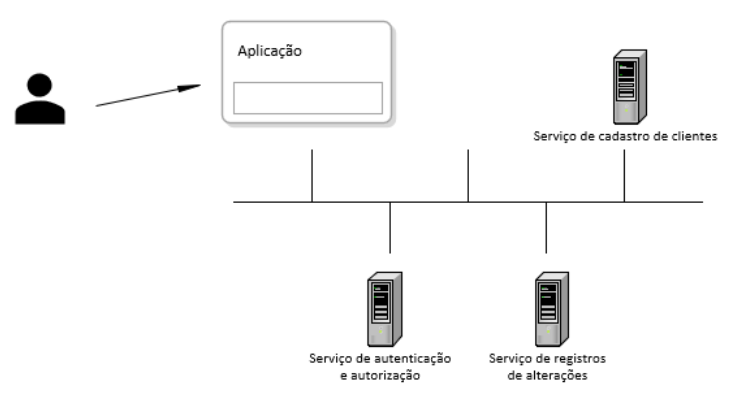
\includegraphics[width=.7\textwidth]{figura1}
  \caption{Barramento de uma aplicação SOA.\label{fig:barramento-de-uma-aplicacao-soa}}
\end{figure}

Na figura 2.1 encontra-se um diagrama simplificado de uma aplicação hipotética onde
a interface com o usuário se comunica com vários serviços como: autenticação e
autorização, cadastro de clientes e registros de alterações.

Para um usuário realizar alterações nos dados de um cliente ele irá utilizar a
interface da aplicação, que por sua vez utilizará o serviço de autenticação e
autorização para validar a identidade do usuário e se este possui as permissões
necessárias para a alteração.

Em seguida, uma chamada ao serviço de cadastro de clientes será feita para realizar
as alterações necessárias e por fim o serviço de registro de alterações será
acionado para registrar que o usuário autenticado realizou uma alteração no
cadastro de um cliente.

Com este exemplo é possível mostrar como vários serviços independentes podem ser
utilizados para compor um sistema de software modular e de baixo grau de acoplamento.

\section{Noções em escalabilidade e resiliência}
\label{sec:nocoes-em-escalabilidade-e-resiliencia}

Para que um sistema de software obtenha sucesso, ele precisa ter um grande número de
usuários, e estes precisam estar satisfeitos com seu desempenho e disponibilidade.
Estes dois requisitos não funcionais dependem de duas características do software:
escalabilidade e resiliência.

A escalabilidade se traduz na capacidade de conseguir atender desde um pequeno
número de usuários até centenas de milhares deles. Já a resiliência é caracterizada
pela capacidade do sistema de se manter operante mesmo diante de falhas, sejam estas
dentro ou fora de sua infraestrutura, que em algum momento irão ocorrer.

A escalabilidade de um sistema de software é habitualmente endereçada com a adição
de novos recursos computacionais. A adição destes recursos pode ser tanto na forma
vertical, com o aumento de recursos como processador e memória para uma instância do
sistema em execução, como horizontal, adicionando mais máquinas ao sistema.

Já a resiliência por sua vez está atrelada com a arquitetura do sistema, a qual
deverá prever que em algum momento as máquinas, conexões de rede, ou até mesmo um
\textit{data-center} inteiro poderão falhar. Com a arquitetura adequada, é possível
criar um sistema de software que atenda ambas as necessidades de escalabilidade e
resiliência.

No diagrama abaixo (figura 2.2) encontra-se um exemplo simplificado de arquitetura de
um sistema de software executado em vários servidores, os quais estão localizados
em dois \textit{data-centers} fisicamente separados, atendendo diversos usuários que
irão se conectar a estes servidores através de balanceadores de carga.

\begin{figure}
  \centering
  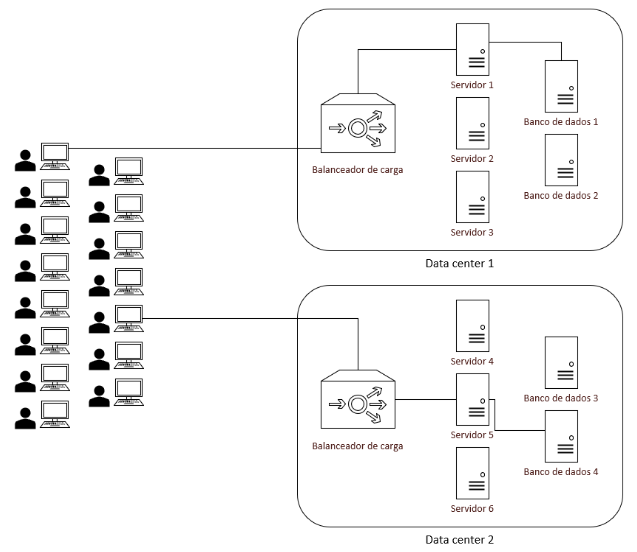
\includegraphics[width=.7\textwidth]{figura2}
  \caption{Diagrama de aplicação resiliente.\label{fig:diagrama-de-aplicacao-resiliente}}
\end{figure}

Alguns detalhes, como replicação de bancos de dados e mecanismos de direcionamento
dos usuários aos balanceadores de carga, estão ocultos nesta visualização, mas de
forma simplificada é desta maneira que um sistema de software deve ser arquitetado
para que os requisitos de escalabilidade e resiliência sejam atendidos.

\section{Balanceadores de carga}
\label{sec:balanceadores-de-carga}

Os balanceadores de carga são peças chave para que um sistema de software possa ser
escalável e resiliente (mais informações em \emph{Availability and Load Balancing in Cloud Computing}~\citep{chaczko}).
Estes componentes atuam intermediando as requisições dos usuários para os servidores,
direcionando as requisições somente para servidores que estejam em pleno funcionamento.

A resiliência é garantida pois, se um destes servidores deixar de funcionar, ele não
receberá mais requisições do balanceador de carga e também, se um dos balanceadores
de carga deixar de funcionar, um outro balanceador poderá continuar fazendo o
redirecionamento de requisições para todos os servidores ativos.

É importante notar que nunca deve haver somente um balanceador de carga, pois ele
iria comprometer totalmente a disponibilidade da aplicação em caso de falha.

\section{Micro-serviços, containers e Kubernetes}
\label{sec:micro-servicos-containers-e-kubernetes}

Com a computação em nuvem e o conceito de infraestrutura como código, o modelo de
arquitetura SOA evoluiu para o que atualmente conhecemos como micro-serviços, o
qual se diferencia principalmente pela independência na implantação de cada serviço.

O principal motivo para sua popularidade é a facilidade que cada micro-serviço
passou a ter para definição suas necessidades de servidores, balanceadores de
carga e bancos de dados, através de arquivos texto que são processados por
mecanismo de automação na sua implantação.

Na figura 2.3 é possível ver um exemplo de como uma aplicação pode ser composta de
vários micro-serviços, executados de forma independente, mas com dependências
entre si.

\begin{figure}
  \centering
  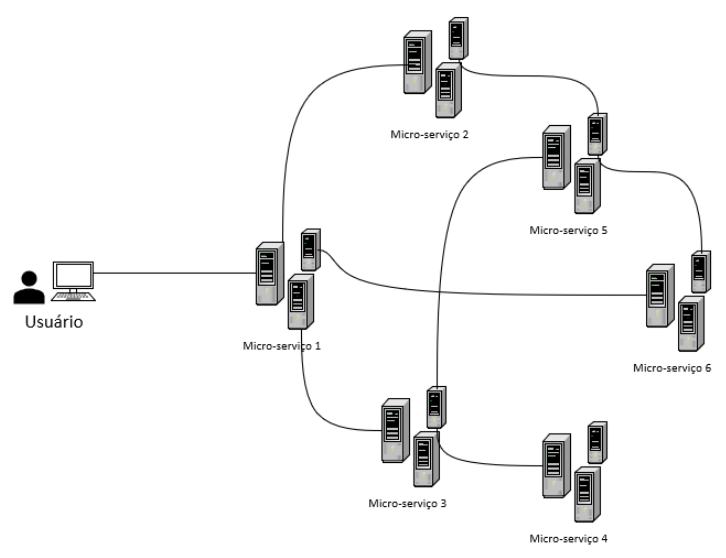
\includegraphics[width=.7\textwidth]{figura3}
  \caption{Diagrama de micro-serviços.\label{fig:diagrama-de-micro-servicos}}
\end{figure}

Como os micro-serviços que tratamos neste documento são aplicações que se
comunicam por uma rede utilizando geralmente o protocolo HTTP, estes também são
conhecidos como aplicações web.

Outro fator que posteriormente contribuiu ainda mais para a maior adoção desta
arquitetura foram os containers Linux e sistemas de orquestração e gerenciamento
de containers.

Os containers Linux permitem que um processo seja executado como se ele estivesse
em uma máquina exclusiva, isolando bibliotecas dos quais ele depende e também
oferecendo uma inicialização muito mais rápida que uma máquina virtual visto que
o núcleo do sistema operacional é compartilhado pelos vários containers e este já
está pronto para ser utilizado quando se inicia um container novo.

Para facilitar a gerência na execução de containers Linux foram criados diversos
projetos como o Kubernetes\footnote[4]{\url{http://kubernetes.io}}, desenvolvido
pela Google, e o Docker Swarm\footnote[5]{\url{docs.docker.com/engine/swarm}},
desenvolvido pela Docker Inc., também responsável pela implementação de
containers Linux denominada Docker\footnote[6]{\url{www.docker.com/resources/what-container}}.

Com a utilização destes projetos, é possível gerenciar automaticamente um conjunto
de máquinas para a execução de diversos containers de micro-serviços, garantindo
a reinicialização da aplicação em caso de falha, e escalabilidade, iniciando
novos containers nas máquinas conforme a necessidade.

\section{Detecção de falhas}
\label{sec:deteccao-de-falhas}

Para realizar uma análise de um sistema de software implantado utilizando a
arquitetura de micro-serviços, independente de sua infraestrutura de implantação,
esta pesquisa propõe uma análise não invasiva dos serviços utilizando somente os
registros dos balanceadores de carga a frente dos micro-serviços.

Os registros dos balanceadores de carga contém informações bastante interessantes
como os horários que as requisições iniciaram e foram concluídas, além de
quantidades de dados trafegados, o serviço que foi acessado e o tempo que este
serviço levou para ser executado. Estes dados devem ser suficientes para se
traçar um perfil de comportamento, permitindo detectar casos que fugiram deste
perfil e analisá-los com mais detalhes.

\section{Classificação de falhas}
\label{sec:classificacao-de-falhas}

Uma vez que as falhas podem ser detectadas, estas podem ser classificadas
conforme sua causa raiz, que pode variar desde um excesso de utilização a uma
falha de um banco de dados, por exemplo.

Com experimentos provocando falhas simuladas, é possível realizar o treinamento
de um algoritmo de aprendizado de máquina para que novas falhas de aplicações
reais possam ser classificadas, permitindo inferir a causa provável de um
problema na aplicação.

O objetivo final desta pesquisa é de detectar e classificar uma falha em um
serviço o quanto antes pois, dado o cenário complexo de micro-serviços exposto
acima, uma falha em uma aplicação pode causar impactos em outras aplicações,
o que poderia causar problemas maiores para todo o sistema de software.

\par

%!TeX root=../tese.tex

%% ------------------------------------------------------------------------- %%
\chapter{Metodologia}
\label{cap:metodologia}

Neste capítulo será detalhado o método que se deseja utilizar para realizar a
detecção de anomalias que esta pesquisa propõe.

Para a análise do comportamento da aplicação serão coletados dados de aplicações
web de forma não invasiva. O principal motivo para utilizar estes dados está na
facilidade com que eles podem ser obtidos sem a necessidade que as aplicações
tenham que ser instrumentadas para dar informações de seu comportamento.

Para obtenção destes dados serão utilizados registros das requisições e respostas
intermediadas por balanceadores de carga, os quais contém o mínimo de informação
necessária para a avaliação proposta, e tratando assim a aplicação como uma caixa
preta (figura 3.1) da qual não precisamos conhecer nenhum detalhe interno.

\begin{figure}
  \centering
  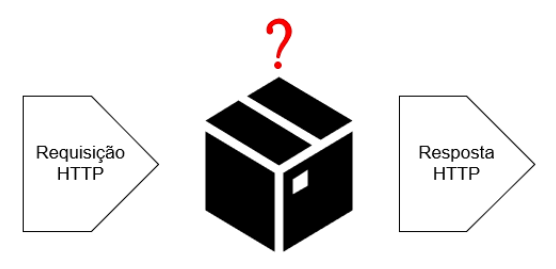
\includegraphics[width=.7\textwidth]{figura4}
  \caption{Aplicação tratada como uma caixa preta.\label{fig:aplicacao-tratada-como-uma-caixa-preta}}
\end{figure}

Outro motivo para esta abordagem é a possibilidade deste mecanismo ser genérico o
suficiente para se tornar um serviço de monitoramento de outros serviços, o que é
bastante interessante para a empresa HP Inc., da qual sou funcionário, que irá
fornecer dados de aplicações em produção para realização de testes.


Na figura 3.2 é descrita a arquitetura de uma aplicação real que realiza o
armazenamento de arquivos em diversos provedores.

\begin{figure}
  \centering
  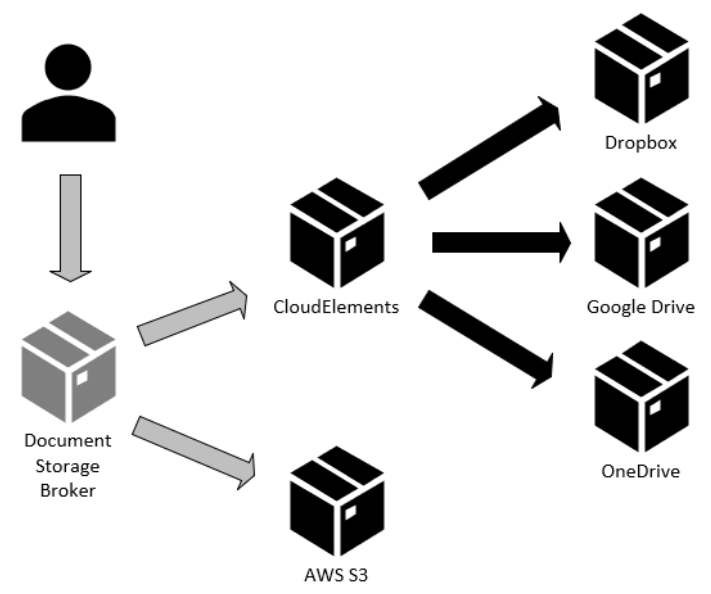
\includegraphics[width=.7\textwidth]{figura5}
  \caption{Interação entre serviços do \textit{Document Storage Broker}.\label{fig:document-storage-broker}}
\end{figure}

O serviço Document Storage Broker recebe requisições dos usuários e encaminha para
o serviço de outra empresa chamada CloudElements\footnote[7]{\url{http://www.cloud-elements.com}},
intermediária de outros serviços como Dropbox, Google Drive ou OneDrive, ou para o
serviço de armazenamento de arquivos da AWS, conforme parâmetros enviados pelo
usuário.

Nesta arquitetura seria possível utilizar a metodologia apresentada tanto nas
requisições recebidas pelo Document Storage Broker quanto nas que são enviadas
para as empresas CloudElements e AWS.

De posse destes dados serão utilizadas técnicas de aprendizado de máquina de
detecção de anomalias e regressão logística para tentar responder às seguintes
questões:

\begin{enumerate}
  \item A aplicação web está se comportando de forma anômala?
  \item Qual a causa provável da anomalia?
\end{enumerate}

Alguns cenários esperados para anomalia e causa são: aumento de tempo de resposta
dado um aumento no número de usuários acessando a aplicação, e aumento na
quantidade de erros dada uma falha em uma dependência da aplicação.

Os dados a serem avaliados inicialmente serão provenientes de uma aplicação de
teste com cenário de sobrecarga e posteriormente serão realizados testes utilizando
dados anonimizados de uma aplicação em produção da empresa HP Inc., os quais estão
pendentes de autorização da empresa para sua publicação.

Caso não seja permitida a publicação dos registros da HP Inc., serão publicados
registros novos da aplicação de teste que irão simular os cenários que desejamos
detectar.

\par

%!TeX root=../tese.tex

%% ------------------------------------------------------------------------- %%
\chapter{Proposta de trabalho}
\label{cap:proposta-de-trabalho}

Inicialmente partiremos de registros de requisições processadas por uma aplicação
de teste para detectar e analisar anomalias que tenham acontecido durante o tempo
em que os registros foram coletados. Posteriormente, será implementado um modelo
onde esta análise ocorrerá de forma contínua, com um período de aprendizado no
início seguido do aprimoramento constante conforme a aplicação é utilizada.

Para a avaliação da aplicação de teste as seguintes etapas serão necessárias:

\begin{enumerate}
  \item Coleta de registros de requisições;
  \item Filtragem dos registros de requisições;
  \item Agregação de registros e extração de novas características;
  \item Avaliação da URL acessada;
  \item Treinamento dos modelos;
  \item Detecção de caso anômalo;
  \item Avaliação de melhoria contínua do treinamento inicial;
  \item Classificação de caso anômalo;
  \item Agregação de casos anômalos classificados.
\end{enumerate}

\section{Etapa 1 - Coleta de registros de requisições}
\label{sec:etapa-1}

Os registros das requisições processadas serão extraídos a partir de balanceadores
de carga conforme o diagrama abaixo sem adicionar complexidade ou atraso na resposta
do serviço uma vez que os balanceadores de carga já são elementos necessários para
garantir a alta disponibilidade de uma aplicação web.

\begin{figure}
  \centering
  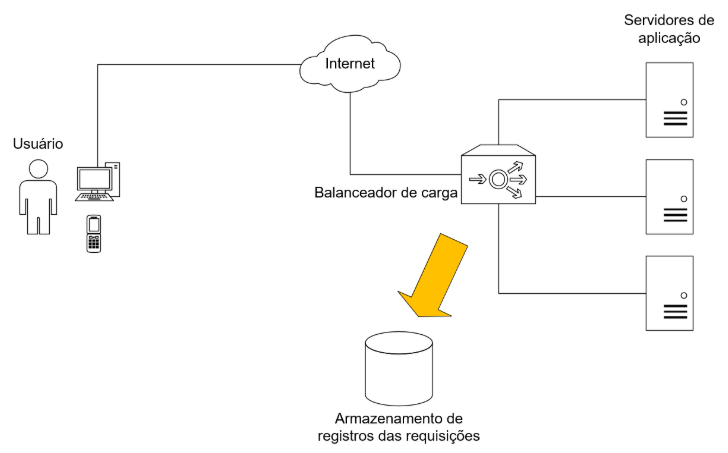
\includegraphics[width=.7\textwidth]{figura6}
  \caption{Extração de dados de balanceadores de carga.\label{fig:extracao-de-dados-de-balanceadores-de-carga}}
\end{figure}

Existem muitas opções de balanceadores de carga possíveis, entretanto as informações
abaixo relacionadas estão presentes nas principais aplicações ou serviços utilizados
como balanceadores de carga (por exemplo: Nginx\footnote[8]{\url{http://www.nginx.com}},
HA-Proxy\footnote[9]{http://www.haproxy.org}, AWS Application Load 
Balancer\footnote[10]{http://aws.amazon.com/elasticloadbalancing}):

\begin{itemize}
  \item Data e hora da solicitação;
  \item URL solicitada;
  \item Verbo HTTP utilizado;
  \item Instância/máquina que realizou o processamento;
  \item Quantidade de bytes recebidos;
  \item Quantidade de bytes enviados;
  \item Tempo de processamento;
  \item Código de resposta HTTP.
\end{itemize}

Como cada balanceador de carga tem seu formato de registro de uma requisição
intermediada, estes registros serão convertidos em um formato padrão que será
utilizado pelas etapas seguintes.

\section{Etapa 2 - Filtragem dos registros de requisições}
\label{sec:etapa-2}

Esta etapa é necessária para filtrar eventuais registros indesejados dos
balanceadores de carga pois eventualmente o balanceador de carga pode ser
responsável por mais de uma aplicação web, e seus registros podem conter
dados que não desejamos tratar.

Também existem registros de falhas indeterminadas, ou com ausência das
informações apontadas na etapa 1, que desejamos remover para evitar ruídos
nos dados.

O caso específico de falha na comunicação entre o balanceador de carga e a
aplicação deverá ter o código de resposta HTTP mapeado para zero para que
este cenário importante possa ser detectado, pois pode sinalizar falhas em
uma instância.

\section{Etapa 3 - Agregação e extração de características dos registros
         para o aprendizado de máquina}
\label{sec:etapa-3}

Nesta etapa será extraída a informação de taxa de requisições concorrentes,
que não fazem parte de um registro isolado, mas dependem de um conjunto de
registros que estavam sendo processados no mesmo espaço de tempo.

Tomando uma janela de tempo fixa, ou de acordo com o tempo que a requisição
levou para ser processada, podemos recuperar a taxa de requisições a qual a
aplicação web estava sendo submetida.

Para o cálculo deste valor será utilizado como identificador somente a
identificação da instância que processou a requisição, independente de verbo
HTTP e URL, uma vez que desejamos saber a taxa de requisições concorrentes da
instância e não de uma requisição específica.

A mesma abordagem pode ser utilizada para o tráfego de dados para tentar
identificar que o gargalo na execução de uma requisição são as interfaces de
comunicação com a rede, porém por não ser certo que os bytes trafegados foram
distribuídos uniformemente durante o intervalo de tempo da requisição esta
métrica será deixada de lado neste momento.
 
Para a recuperação da taxa de requisições concorrentes será implementado um
contador de requisições ativas para cada janela de 1 segundo, e durante o
intervalo de tempo em que a requisição esteve ativa os contadores serão
incrementados. O intervalo de 1 segundo é o que se espera ser o mais adequado,
entretanto durante a execução da pesquisa será avaliado se este valor é de
fato o mais adequado.

\begin{figure}
  \centering
  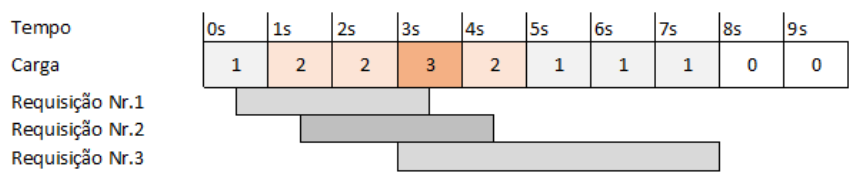
\includegraphics[width=.8\textwidth]{figura7}
  \caption{Carga de requisições ao longo do tempo.\label{fig:carga-de-requisicoes-ao-longo-do-tempo}}
\end{figure}

Adicionalmente serão extraídas novas características para o valor de resposta
HTTP dado que um modelo de aprendizado de máquina não conseguiria estabelecer
uma relação linear para os códigos de retorno. Para isto serão isolados em
características distintas e mapeados de acordo com a tabela abaixo:

\begin{table}[H]
\centering
\caption{Mapeamento de respostas HTTP para um vetor.}
\vspace{0.25cm}
\begin{tabular}{ll}
Resposta HTTP & Vetor de características            \\
\hline
0	      &	[0, 0, 0, 0, 0]                         \\
100 a 199 &	[1000, 0, 0, 0, 0] a [1099, 0, 0, 0, 0] \\
200 a 299 &	[0, 1000, 0, 0, 0] a [0, 1099, 0, 0, 0] \\
300 a 399 &	[0, 0, 1000, 0, 0] a [0, 0, 1099, 0, 0] \\
400 a 499 &	[0, 0, 0, 1000, 0] a [0, 0, 0, 1099, 0] \\
500 a 599 & [0, 0, 0, 0, 1000] a [0, 0, 0, 0, 1099]
\end{tabular}
\end{table}

Acima estão sendo utilizados os valores de dois parâmetros que serão ajustados
posteriormente de acordo com os resultados dos testes. São estes:

\begin{table}[H]
\caption{Parâmetro $H_{min}$.}
\vspace{0.25cm}
\begin{tabular}{ll}
Parâmetro      & $H_{min}$ \\
Valor proposto & 1000 \\
Descrição      & Valor mínimo caso a categoria de respostas HTTP esteja ativa.
\end{tabular}
\end{table}

\begin{table}[H]
\caption{Parâmetro $H_{range}$.}
\vspace{0.25cm}
\begin{tabular}{ll}
Parâmetro      & $H_{range}$ \\
Valor proposto & 100 \\
Descrição      & Valor para o qual os valores da categoria X, de X00 a X99 deverão \\
               & ter sua escala ajustada.
\end{tabular}
\end{table}

Ou seja, o vetor de características $R_{vector}$ para um código de resposta R poderia ser gerado com:

\begin{program}
  \centering
  \begin{lstlisting}[language=Java, style=wider]
    int[] getRVector(int R, int hMin, int hRange) {
        int[] rVector = new int[] { 0, 0, 0, 0, 0 };
        if (R > 100) {
            rVector[ (int) Math.floor( R / 100 ) - 1 ] = hMin + (int) ((float) (R \% 100) / 100 * hRange);
        }
	    return rVector;
	}
  \end{lstlisting}
  \caption{Código para cálculo do vetor $R_{vector}$.\label{prog:java}}
\end{program}

Os valores 1000 e 100 estão sendo utilizados para que o valor 0, que representa
a não ocorrência daquela característica, esteja suficientemente distante e que
permita ainda as variações dentre a categoria de resposta serem detectadas.
O valor 0 que representa ausência de resposta HTTP está sendo mapeado para um
vetor zero que difere bastante dos outros valores em caso de resposta.

Posteriormente será avaliada a necessidade de normalizar as características
coletadas para que a detecção seja mais eficiente, porém neste momento da
pesquisa esta etapa aparenta não ser necessária.

Também será analisada a ideia de se isolar códigos de erro específicos que
indiquem algum cenário, como por exemplo:

\begin{itemize}
  \item 401 (Unauthorized) e 403 (Forbidden): Indicam falhas relacionadas a permissão de acesso;
  \item 502 (Bad Gateway) e 504 (Gateway timeout): Indicam possíveis falhas com serviços do qual a aplicação depende.
\end{itemize}

\section{Etapa 4 - Avaliação da URL acessada}
\label{sec:etapa-4}

Esta etapa determina como a URL será utilizada para ter seus registros agrupados
em uma forma que seja possível determinar quais URLs correspondem a um determinado
serviço da aplicação web.

Existe um problema crítico na utilização da uma URL para identificar um tipo de
serviço, visto que identificadores de recursos são bastante comuns em parte do
caminho acessado. Por exemplo, em uma aplicação de cuida de cadastros de clientes
pode ter requisições como as abaixo:

\begin{table}[H]
\centering
\caption{Exemplos de requisições HTTP.}
\vspace{0.25cm}
\begin{tabular}{ll}
Verbo & Caminho do recurso \\
\hline
POST & /clientes           \\
GET  & /clientes/42        \\
PUT  & /clientes/42        \\
GET  & /clientes/99        \\
GET  & /clientes/999       \\
GET  & /health
\end{tabular}
\end{table}

Das requisições acima relacionadas, as de verbo ``GET'' para o caminho
``/clientes/\{número\}'' são bastante parecidas e provavelmente devem executar um
código de recuperação de dados do cliente identificado pelo número.

Para agrupar estes dados será utilizada uma estrutura de árvore com os caminhos
acessados e os nós mais ``comuns'' terão uma quantidade de registros maior que os
demais.

\begin{figure}
  \centering
  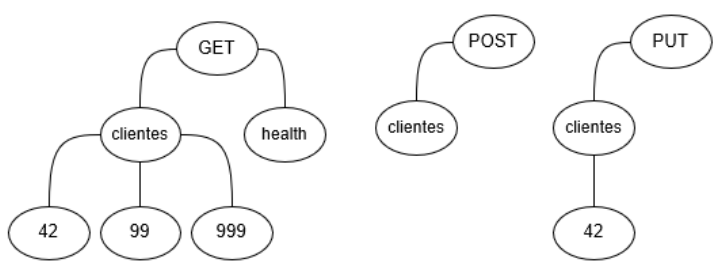
\includegraphics[width=.7\textwidth]{figura8}
  \caption{Caminho da URL em uma árvore.\label{fig:caminho-da-url-em-uma-arvore}}
\end{figure}

Ao receber um registro de uma requisição a árvore será percorrida e os nós que
fazem parte do caminho deste registo terão uma referência para este registro,
desta forma será possível avaliar quais são os nós que tem relevância para agrupar
registros por um número suficientemente grande de referências, porém com nós filhos
com poucas referências.

Será avaliada também a ideia de utilizar expressões regulares para definir os
serviços monitorados, pois em alguns cenários a utilização do caminho inicial comum
pode não ser suficiente para identificar o grupo de requisições.

\section{Etapa 5 - Treinamento dos modelos}
\label{sec:etapa-5}

Uma vez que as etapas anteriores já coletaram e processaram os dados das requisições,
o treinamento dos modelos poderá ser iniciado. Caso existam dados salvos de
treinamentos anteriores, eles poderão ser carregados para serem aprimorados com
novos registros.

O treinamento será independente para cada conjunto de verbo HTTP, caminho parcial da
URL e instância monitorada, conforme descrito na etapa 4, desta forma estaremos
monitorando sempre o mesmo código executado da aplicação web apesar de que sua
execução poderá ser diferente de acordo com os parâmetros.

Dado que estamos considerando a instância monitorada, também será possível na etapa
de classificação identificar se as anomalias acontecem em algumas instâncias somente. 

Durante o desenvolvimento desta pesquisa serão avaliados diversos parâmetros que
poderão ser alterados conforme a necessidade. Inclusive descobrir quais parâmetros
deverão ser alterados e para que valores é parte do desafio de pesquisa. São estes:

\begin{table}[H]
\caption{Parâmetro $N_{min}$.}
\vspace{0.25cm}
\begin{tabular}{ll}
Parâmetro      & $N_{min}$ \\
Valor proposto & 1000 \\
Descrição      & Número mínimo de registros que deverão ser utilizados no \\
               & treinamento de um modelo.
\end{tabular}
\end{table}

\begin{table}[H]
\caption{Parâmetro $T_{min}$.}
\vspace{0.25cm}
\begin{tabular}{ll}
Parâmetro      & $T_{min}$ \\
Valor proposto & 86400 \\
Descrição      & Tempo mínimo em segundos que as requisições devem ser \\
               & coletadas para um treinamento sem dados prévios.
\end{tabular}
\end{table}

A etapa de detecção de anomalias irá se basear em avaliação de probabilidade em uma
distribuição multivalorada gaussiana (mais informações em \citep{ng}), que será
treinada uma vez que ambos os critérios de $N_{min}$ e $T_{min}$ sejam obedecidos.

Assim que houver a quantidade de amostras necessária, as fórmulas abaixo serão
aplicadas para $m$ registros $x_i$ e os valores de $\mu$ e $\Sigma$ corresponderão ao
treinamento para estes registros.

\begingroup
\Large
\begin{equation}
\displaystyle \mu = \frac{1}{m} \sum_{i=1}^{m} x_i , \mu \in \mathbb{R}^d
\end{equation}
\endgroup

\begingroup
\Large
\begin{equation}
\displaystyle \Sigma = \frac{1}{m} \sum_{i=1}^{m} \left[ ( x_i - \mu ) ( x_i - \mu )^{T} \right] , \Sigma \in \mathbb{R}^{d \times d}
\end{equation}
\endgroup

\section{Etapa 6 - Detecção de caso anômalo}
\label{sec:etapa-6}

Para a detecção de caso anômalo será calculada a probabilidade $p(x_i)$ de um caso $x_i$
ser semelhante aos casos observados no cálculo de $\mu$ e $\Sigma$, e o valor limite será
definido através do parâmetro $P_{min}$.

\begin{table}[H]
\caption{Parâmetro $P_{min}$.}
\vspace{0.25cm}
\begin{tabular}{ll}
Parâmetro      & $P_{min}$ \\
Valor proposto & 0.25 \\
Descrição      & Probabilidade mínima requerida para que o registro sob análise \\
               & não seja considerado anômalo.
\end{tabular}
\end{table}

Caso a probabilidade $p(x_i)$ seja menor que $P_{min}$ a ocorrência $x_i$ será
classificada como anômala e passará pela etapa de classificação (etapa 8).

\begingroup
\Large
\begin{equation}
p(x_i; \mu, \Sigma) = \frac{1}{(2 \pi)^{\frac{n}{2}} | \Sigma |^{\frac{1}{2}} } exp \left( - \frac{1}{2} ( x_i - \mu )^{T} \Sigma^{-1} ( x_i - \mu ) \right)
\end{equation}
\endgroup

\section{Etapa 7 - Melhoria contínua do treinamento inicial}
\label{sec:etapa-7}

O treinamento inicial será realizado assim que houver a quantidade mínima de
registros necessários, entretanto após este treinamento inicial ser realizado,
o modelo definido por $\mu$ e $\Sigma$ deverá ser atualizado de regularmente
com todos os novos registros observados, tenham estes sido classificados como
anômalos ou não.

\begin{table}[H]
\caption{Parâmetro $T_{update}$.}
\vspace{0.25cm}
\begin{tabular}{ll}
Parâmetro      & $T_{update}$ \\
Valor proposto & 1800 \\
Descrição      & Tempo mínimo em segundos para que novos registros sejam considerados \\
               & no novo treinamento do modelo.
\end{tabular}
\end{table}

\begin{table}[H]
\caption{Parâmetro $P_{update}$.}
\vspace{0.25cm}
\begin{tabular}{ll}
Parâmetro      & $P_{update}$ \\
Valor proposto & 0.02 \\
Descrição      & Percentual em que os novos registros irão influenciar um modelo \\
               & treinado.
\end{tabular}
\end{table}

De forma paralela a detecção, um algoritmo de atualização será executado a
cada $T_{update}$ segundos para atualização dos valores $\mu$ e $\Sigma$ com $n$
novas amostras coletadas. As fórmulas utilizadas na etapa 5 serão alteradas de
forma que os novos registros tenham um peso limitado sobre os valores de $\mu$
e $\Sigma$ atuais, conforme abaixo:

\begingroup
\Large
\begin{equation}
\displaystyle \mu ' = (1 - P_{update} ) \mu + P_{update} \frac{1}{n} \sum_{i=1}^{n} x_i
\end{equation}
\endgroup

\begingroup
\Large
\begin{equation}
\displaystyle \Sigma ' = (1 - P_{update} ) \Sigma + P_{update} \frac{1}{n} \sum_{i=1}^{n} \left[ ( x_i - \mu ' ) ( x_i - \mu ' )^{T} \right]
\end{equation}
\endgroup

A importância de se limitar o quanto os novos registros irão afetar o treinamento
é de impedir que uma falha que dure vários minutos possa influenciar no
aprendizado de forma que estas falhas deixem de ser detectadas. Adicionalmente
também é importante limitar a influência de registros antigos para que mudanças
na aplicação possam influenciar o treinamento existente.

\section{Etapa 8 - Classificação de caso anômalo}
\label{sec:etapa-8}

Para a classificação do caso anômalo será utilizado o valor de $\delta_i = ( x_i - \mu )$
como dado de entrada pois ele representa o quanto cada característica diferiu do valor
médio esperado para ela.

Os vetores $\delta_i$ serão eventualmente pré-processados para normalizar os valores e
utilizando um algoritmo de regressão logística (mais informações em \citep{mostafa}),
ou outro mecanismo de aprendizado de máquina supervisionado, serão classificados como
algum dos tipos de falha abaixo:

\begin{itemize}
  \item Aplicação sobrecarregada;
  \item Aplicação sobrecarregada e irresponsiva;
  \item Falha em dependência da aplicação.
\end{itemize}

Dado que a ocorrência de falhas nas aplicações web não é algo frequente, serão
simulados alguns cenários com uma aplicação de teste para realizar o treinamento
deste modelo de aprendizado de máquina. A aplicação de teste será submetida aos
seguintes cenários:

\begin{enumerate}
  \item Aumento de carga além do esperado provocando um aumento no tempo de
        resposta mas sem gerar erros. Os resultados anômalos detectados serão
		classificados como ``Aplicação sobrecarregada'';
  \item Aumento de carga além do esperado provocando um aumento no tempo de
        resposta gerando erros, ou vindos da aplicação ou do balanceador de carga.
		Os resultados anômalos detectados serão classificados como ``Aplicação
		sobrecarregada e irresponsiva'';
  \item Remoção de dependência, como um banco de dados, provocando erros na resposta
        da aplicação. Os resultados anômalos serão classificados como ``Falha em
		dependência da aplicação''.
\end{enumerate}


\section{Etapa 9 - Agregação de casos anômalos classificados}
\label{sec:etapa-9}

Uma vez que as anomalias forem classificadas, será necessário avaliar a quantidade
de anomalias, para avaliar casos isolados, se elas foram classificadas da mesma
forma ou se são classificações variadas e ainda se é uma única instância que está
sofrendo desta anomalia ou várias delas.

Os resultados previstos a serem reportados são:

\begin{itemize}
  \item Nenhuma anomalia
  \item Pequenas anomalias detectadas
  \item Instância defeituosa
  \item Aplicação sobrecarregada
  \item Aplicação sobrecarregada e irresponsiva
  \item Falha em dependência da aplicação
  \item Falha geral na aplicação.
\end{itemize}

O parâmetro $A_{min}$ será utilizado para definir se o resultado final da análise
será de ``Pequenas anomalias detectadas'', indicando que algo anormal foi detectado
mas não tem relevância suficiente para disparar algum alarme ou ação automática.
Abaixo segue a definição deste parâmetro:

\begin{table}[H]
\caption{Parâmetro $A_{min}$.}
\vspace{0.25cm}
\begin{tabular}{ll}
Parâmetro      & $A_{min}$ \\
Valor proposto & 0.01 \\
Descrição      & Percentual mínimo de requisições anômalas para \\
               & que estas sejam apontadas.
\end{tabular}
\end{table}

Uma vez que a quantidade de anomalias sejam significantes deverá ser avaliado se
somente uma instância está sendo afetada. Em caso positivo o resultado final da
análise será de ``Instância defeituosa''.

Caso múltiplas instâncias sejam afetadas o resultado final da análise será dado
pela classificação que tenha mais de 50\% das ocorrências e caso não exista uma
que possua esta quantidade o resultado reportado deverá ser de ``Falha geral na
aplicação''. Este percentual inicialmente não será parametrizado, porém conforme
resultados da pesquisa ele poderá ser alterado.

\par

%!TeX root=../tese.tex

%% ------------------------------------------------------------------------- %%
\chapter{Experimento preliminar}
\label{cap:experimento-preliminar}

Foi realizado um experimento de teste utilizando a nuvem pública de computação
da Amazon Web Services usando uma máquina virtual EC2 com 1 vCPU e 1GB de
memória RAM. Para ter o cenário de um balanceador de carga na frente da
aplicação foi criado um Application Load Balancer direcionando o tráfego
HTTP para esta máquina e coletando os registros das requisições no serviço
de armazenamento S3.

\begin{figure}
  \centering
  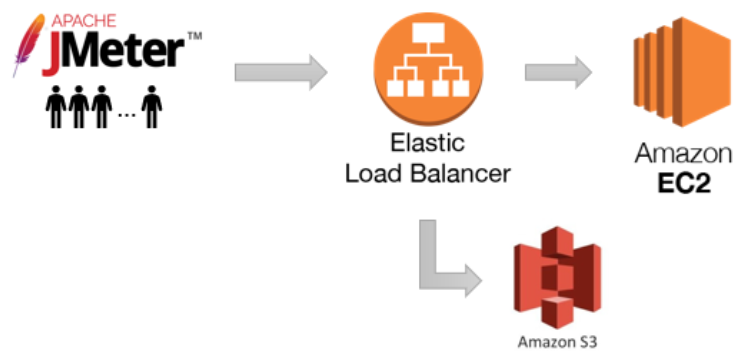
\includegraphics[width=.7\textwidth]{figura9}
  \caption{Diagrama do experimento preliminar.\label{fig:diagrama-do-experimento-preliminar}}
\end{figure}

A aplicação web foi criada utilizando SpringBoot atendendo requisições GET
que executavam o código Java abaixo, consumindo tanto CPU quanto memória:

\begin{program}
  \centering
  \begin{lstlisting}[language=Java, style=wider]
    List<Integer> array = new ArrayList<>();
    for (int index = 0; index < 1000000; index++) {
      array.add((int) (Math.random() * Integer.MAX_VALUE));
    }
    Collections.sort(array);
  \end{lstlisting}
  \caption{Código de teste da aplicação web.\label{prog:java}}
\end{program}

O teste da aplicação foi feito utilizando JMeter para com o número de usuários
concorrentes variando ao longo do tempo chegando a 10 usuários concorrentes.

\begin{figure}
  \centering
  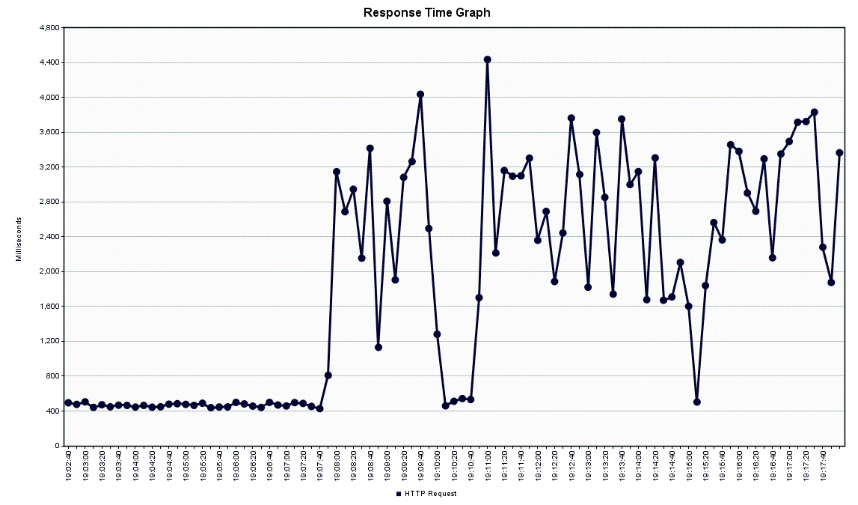
\includegraphics[width=.7\textwidth]{figura10}
  \caption{Tempo de resposta da aplicação ao longo do tempo.\label{fig:tempo-de-resposta-da-aplicação-ao-longo-do-tempo}}
\end{figure}

A figura acima mostra o tempo de resposta da requisição ao longo da execução
do teste. A aplicação se comporta bem no início, porém após os créditos de
CPU da instância se esgotarem ela começa a ter tempos de resposta bastante
altos, e será justamente esta anomalia que desejamos identificar neste
experimento.

Os créditos de CPU mencionados são uma forma da AWS permitir que a máquina
utilize um pouco mais de CPU durante picos de uso, pois créditos de CPU são
incrementados até um certo limite caso a máquina esteja ociosa, ou
consumidos em caso de alta carga.

Foram coletados 565 registros do ALB correspondentes a este teste e algumas
amostras estão nas tabelas abaixo, onde os valores das colunas correspondem a:

\begin{enumerate}
  \item Data e hora do início da requisição no ALB no formato ISO-8601;
  \item Data e hora do término da requisição no ALB no formato ISO-8601;
  \item Instância de destino que executou a requisição;
  \item Tempo de processamento da requisição no destino;
  \item Código de resposta HTTP;
  \item Quantidade de bytes enviados a aplicação;
  \item Quantidade de bytes recebidos da aplicação;
  \item Verbo HTTP utilizado pela requisição;
  \item Caminho da URL utilizado na requisição.
\end{enumerate}

\begin{sidewaystable}[H]
\centering
\caption{Exemplos de registros regulares e anômalos do balanceador de carga.}
Estes exemplos são registros regulares:

\vspace{0.25cm}
\begin{tabular}{lllllllll}
1                           & 2                           & 3                 & 4     & 5   & 6   & 7   & 8   & 9     \\
\hline
2019-11-21T21:02:56.898000Z & 2019-11-21T21:02:57.250351Z & 172.31.7.121:8080 & 0.351 & 200 & 292 & 175 & GET & /test \\
2019-11-21T21:02:57.886000Z & 2019-11-21T21:02:58.233481Z & 172.31.7.121:8080 & 0.347 & 200 & 292 & 175 & GET & /test \\
2019-11-21T21:02:58.877000Z & 2019-11-21T21:02:59.220909Z & 172.31.7.121:8080 & 0.343 & 200 & 292 & 175 & GET & /test \\
2019-11-21T21:02:59.868000Z & 2019-11-21T21:03:00.348951Z & 172.31.7.121:8080 & 0.480 & 200 & 292 & 175 & GET & /test \\
2019-11-21T21:03:00.984000Z & 2019-11-21T21:03:01.337323Z & 172.31.7.121:8080 & 0.352 & 200 & 292 & 175 & GET & /test
\end{tabular}

\vspace{2cm}

Estes exemplos foram considerados anômalos:

\vspace{0.25cm}
\begin{tabular}{lllllllll}
1                           & 2                           & 3                 & 4     & 5   & 6   & 7   & 8   & 9     \\
\hline
2019-11-21T21:16:04.811655Z & 2019-11-21T21:16:00.847000Z & 172.31.7.121:8080 & 3.964 & 200 & 328 & 174 & GET & /test \\
2019-11-21T21:16:09.250483Z & 2019-11-21T21:16:05.195000Z & 172.31.7.121:8080 & 4.054 & 200 & 328 & 174 & GET & /test \\
2019-11-21T21:16:13.374715Z & 2019-11-21T21:16:09.344000Z & 172.31.7.121:8080 & 4.030 & 200 & 328 & 174 & GET & /test \\
2019-11-21T21:16:32.603263Z & 2019-11-21T21:16:28.658000Z & 172.31.7.121:8080 & 3.945 & 200 & 328 & 174 & GET & /test \\
2019-11-21T21:16:51.868990Z & 2019-11-21T21:16:47.794000Z & 172.31.7.121:8080 & 4.074 & 200 & 328 & 174 & GET & /test
\end{tabular}
\end{sidewaystable}

Além do aumento no tempo de execução (coluna 3) é possível notar um aumento
discreto no tamanho da quantidade de bytes recebidos, talvez por algum
cabeçalho HTTP adicional, mas ainda não foi investigado o que provocou esta
alteração.

Utilizando os primeiros 300 registros com respostas bem similares para a etapa
de treinamento da distribuição gaussiana multivalorada, marcamos os registros
com menos de 10\% de probabilidade como anômalos e os resultados foram plotados
na figura 5.3.

\begin{figure}
  \centering
  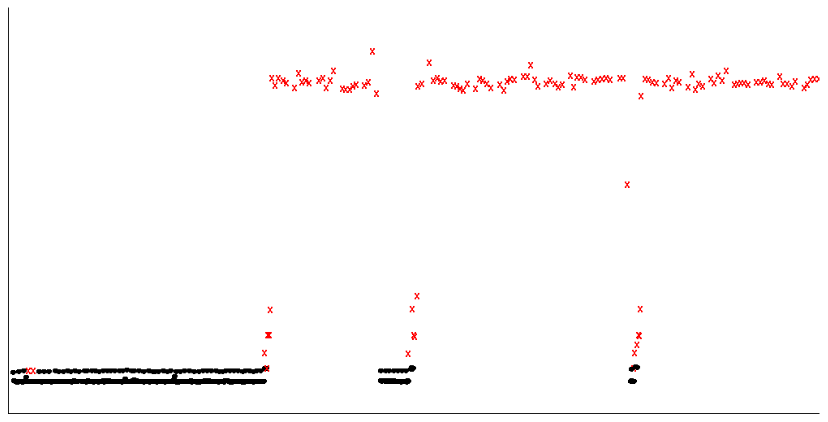
\includegraphics[width=.7\textwidth]{figura11}
  \caption{Anomalias detectadas no experimento.\label{fig:anomalias-detectadas-no-experimento}}
\end{figure}

É possível ver que a classificação de anomalia funciona bem neste cenário controlado
e que alguns registros que deveriam ser considerados normais foram marcados como
anômalos.

Logo no começo é possível ver dois pontos vermelhos que representam duas amostras
que levaram o tempo de 483 e 488 milissegundos enquanto a carga da aplicação
percebida era de 1 execução concorrente. O tempo médio de resposta no
treinamento era de 375 milissegundos e dada a pouca variação ocorrida nos
primeiros 300 registros estes tempos foram marcados como anormais.

Pouco antes de começarem a ocorrer várias falhas com tempos bastante altos foi
detectado um registros com 514 milissegundos de execução. Como a informação de
carga era de que haviam duas execuções concorrentes neste instante a requisição
foi marcada como normal.
 
Com esta observação é possível afirmar que a informação de carga na aplicação estava
de fato sendo considerada na detecção de anomalia, pois a requisição que levou 483
milissegundos no início do teste (sem concorrência) foi identificada como anômala.

\par

%!TeX root=../tese.tex

%% ------------------------------------------------------------------------- %%
\chapter{Trabalhos relacionados}
\label{cap:trabalhos-relacionados}

Foi realizada uma pesquisa por trabalhos semelhantes e a maioria dos trabalhos
encontrados possui diferenças significantes em relação a proposta desta pesquisa.

A busca foi realizada tanto nas buscas gerais do Google quanto no Google Scholar
com as seguintes palavras-chave:

\begin{itemize}
  \item anomaly detection logs
  \item anomaly detection log records
  \item anomaly detection application
  \item anomaly detection application logs
  \item anomaly detection distributed application
  \item anomaly detection http
  \item anomaly detection load balancer
\end{itemize}

Os trabalhos similares encontrados serão detalhados a seguir.

\section{Anomaly Detection for Application Log Data \citep{grover}}
\label{sec:anomaly-detection-for-application-log-data}

Este trabalho possui uma proposta similar de detectar falhas em uma aplicação em
execução de forma não invasiva, detectando anomalias através da saída de texto
da aplicação.

A extração de características é bem diferente e várias abordagens para detecção
de anomalia são propostas, como: detecção baseada em estatística, agrupamento por
similaridade (``clustering''), distância de uma ocorrência ao grupo similar mais
próximo, aprendizado supervisionado e redes neurais.

Esta pesquisa propõe utilizar a detecção baseada em estatística por acreditar que
é o método mais adequado ao cenário, entretanto estas opções serão melhor estudadas
para serem consideradas na escrita da dissertação.

Em relação à classificação, este trabalho se restringe somente a detecção de uma
anomalia na aplicação sem classificá-la, pois a idéia é somente apontar entre as
milhares de linhas de saída da aplicação o que está fora do padrão.

\section{Anomaly Detection in Log Records \citep{rastogi}}
\label{sec:anomaly-detection-in-log-records}

Este outro trabalho também trata da detecção de anomalia baseada em arquivos de
logs de um servidor web Apache, porém com uma abordagem bem mais simplificada.

A detecção de anomalia proposta é sobre a quantidade de requisições HTTP que
partem de uma mesma origem (endereço IP) ao longo do tempo, e o foco da análise
é de predizer estas ocorrências em um futuro próximo.

Apesar da ideia de detecção ser similar, o propósito do artigo é mais focado em
prever o uso futuro dos servidores web, o que é bem distinto desta pesquisa.

\section{PAD: Performance Anomaly Detection in Multi-server Distributed Systems \citep{pad}}
\label{sec:pad}

Esta publicação descreve um software que foi criado para analisar anomalias de
desempenho em aplicações distribuídas que possuem alta demanda e pedem uma baixa
latência de resposta.

Ela difere bastante por ser mais invasiva e requerer contadores de recursos
(CPU, memória e I/O), assim como contadores de mensagens processadas e número de
processos em uma máquina. Adicionalmente ela utiliza uma quantidade destas
características na casa das centenas, o que é computacionalmente caro.

Também é importante ressaltar que o propósito desta aplicação é de ser utilizada
na execução de um teste de desempenho para análise das anomalias e não monitora
o desempenho de uma aplicação em produção como a que esta pesquisa pretende fazer.

\section{Measuring normality in HTTP traffic for anomaly-based intrusion detection \citep{tapiador}}
\label{sec:measuring-normality-in-http-traffic-for-anomaly-based-intrusion-detection}

Neste trabalho o foco está na detecção de intrusão através de anomalias nas
requisições enviadas a uma aplicação web.

A detecção de anomalia é feita de uma forma bastante diferente utilizando cadeias
de Markov para modelar as sequências regulares que a aplicação recebe, marcando
uma sequência de requisições de baixa probabilidade de ocorrência como uma anomalia.

\section{An Anomaly-Based Approach for Intrusion Detection in Web Traffic \citep{TorranoGimnez2010AnAA}}
\label{sec:an-anomaly-based-approach-for-intrusion-detection-in-web-traffic}

Este outro trabalho propõe a criação de um firewall de requisições a aplicações web,
porém ele requer um treinamento manual que descreve o que deve ser considerado
anomalia ou não.

Apesar do título indicar alguma relação com o que está sendo estudado, ele difere
bastante por não aprender automaticamente o que é anomalia ou não, e pela ação de
bloqueio da requisição diante da anomalia percebida.

\section{Performance Anomaly Detection in Microservice Architectures Under Continuous Change \citep{dullmann}}
\label{sec:performance-anomaly-detection-in-microservice-architectures-under-continuous-change}

Esta dissertação de mestrado é a que mais se aproxima do que esta pesquisa propõe
por abordar o contexto de micro-serviços e se basear na performance da aplicação.

Algumas diferenças podem ser apontadas na etapa de detecção de anomalias, a qual
confia em um limiar pré-determinado para apontar quais requisições são anômalas e
nenhuma tentativa de aprendizado do comportamento da aplicação é utilizada.

O autor menciona problemas interessantes que esta pesquisa deve se deparar, como
atrasos iniciais devido a criação de estruturas de dados, cache ou conexões com
bancos de dados na inicialização de uma instância da aplicação. Este cenário será
verificado durante a pesquisa para avaliar se é possível classificá-lo ou suprimir
alertas gerados por este motivo.

\section{Comparativo}
\label{sec:comparativo}

Na tabela 6.1 serão sumarizadas as diferenças entre os trabalhos relacionados
e esta pesquisa: 

Uma vez identificados alguns trabalhos relacionados, temos algumas ideias de
alternativas para detecção de anomalias e também um cenário novo que deverá ser
levado em conta durante os testes do projeto.

Durante o desenvolvimento do projeto e escrita da dissertação, novas pesquisas
serão realizadas para avaliar o surgimento de outros trabalhos relacionados.

É importante ressaltar que esta pesquisa se torna relevante por não haver
nenhuma outra com a mesma proposta, e também por ser de interesse da indústria
de software, uma vez que tenho apoio da empresa HP Inc. na forma de tempo para
inovação e acesso a dados.

\begin{sidewaystable}
\centering
\caption{Comparativo entre trabalhos relacionados e esta pesquisa.}
\begin{tabular}{lcccccc}
Trabalho relacionado             & Utiliza detecção & Utiliza    & Dispensa       & Realiza       & Realiza o        \\
                                 & de anomalia      & logs da    & instrumentação & classificação & monitoramento    \\
                                 & automática       & aplicação  & do código      & de problemas  & de uma aplicação \\
\hline
6.1\citep{grover}                & \checkmark       & \checkmark & \checkmark     &               & \checkmark       \\
6.2\citep{rastogi}               & \checkmark       & \checkmark & \checkmark     &               & \checkmark       \\
6.3\citep{pad}                   & \checkmark       & \checkmark &                &               &                  \\
6.4\citep{tapiador}              & \checkmark       & \checkmark & \checkmark     &               & \checkmark       \\
6.5\citep{TorranoGimnez2010AnAA} &                  & \checkmark & \checkmark     &               & \checkmark       \\
6.6\citep{dullmann}              &                  & \checkmark & \checkmark     & \checkmark    & \checkmark       \\
\end{tabular}
\end{sidewaystable}

\par

%!TeX root=../tese.tex

%% ------------------------------------------------------------------------- %%
\chapter{Cronograma}
\label{cap:cronograma}

O experimento relatado no capítulo 5 indica que a pesquisa proposta é viável,
apesar de ser utilizado um cenário bastante simples, onde só foram realizadas
requisições de um único tipo e os registros não tiveram variação no tipo de
resposta recebida.

Para a escrita da dissertação as seguintes atividades serão necessárias:

\begin{enumerate}
  \item Coleta de registros de um serviço real em ambiente de produção, homologação ou qualificação de aplicações web da empresa HP Inc Brasil;
  \item Realização de testes de detecção de anomalias com os dados do serviço real;
  \item Adequação de algoritmos caso necessário;
  \item Realização de testes de classificação das anomalias detectadas;
  \item Implementação de uma aplicação para fazer o monitoramento de registros de um Application Load Balancer da AWS;
  \item Avaliação da aplicação implementada e coleta de resultados.
\end{enumerate}

As atividades elencadas serão executadas nos próximo 12 meses, iniciando
em janeiro de 2020, conforme a tabela abaixo, com o objetivo de concluir
a dissertação ao final de 2020.

\begin{figure}
  \centering
  \begin{ganttchart}{2020-01}{2020-12}
    \gantttitlecalendar{year,month=shortname} \ganttnewline

    \ganttbar[progress=0]{Atividade 1}{2020-01}{2020-01} \ganttnewline
    \ganttbar[progress=0]{Atividade 2}{2020-02}{2020-03} \ganttnewline
    \ganttbar[progress=0]{Atividade 3}{2020-02}{2020-05} \ganttnewline
	\ganttbar[progress=0]{Atividade 4}{2020-04}{2020-05} \ganttnewline
	\ganttbar[progress=0]{Atividade 5}{2020-06}{2020-08} \ganttnewline
	\ganttbar[progress=0]{Atividade 6}{2020-08}{2020-11} \ganttnewline
	\ganttbar[progress=0]{Dissertação}{2020-06}{2020-12} \ganttnewline
    \ganttmilestone{Submissão}{2020-12}
  \end{ganttchart}

  \caption{Cronograma para conclusão da pesquisa.\label{fig:gantt}}
\end{figure}

\par

\par

%%%%%%%%%%%%%%%%%%%%%%%%%%%%%% SEÇÕES FINAIS %%%%%%%%%%%%%%%%%%%%%%%%%%%%%%%%%%%

% Aqui vão a bibliografia, índice remissivo e outras seções similares.

% O comando backmatter desabilita a numeração de capítulos.
\backmatter

% Este formato está definido na package imeusp-headers
\pagestyle{backmatter}

% Espaço adicional no sumário antes das referências / índice remissivo
\addtocontents{toc}{\vspace{2\baselineskip plus .5\baselineskip minus .5\baselineskip}}

% A bibliografia é obrigatória
\printbibliography[
  title=\refname\label{bibliografia}, % "Referências", recomendado pela ABNT
  %title=\bibname\label{bibliografia}, % "Bibliografia"
  % Inclui a bibliografia no sumário
  heading=bibintoc,
]

\end{document}
